\chapter{$t\bar{t}$ aware reweighting}
\label{app:ttbar-rw}

\section{Motivation}

As shown in \Tab{\ref{tab:ttbar-proportion}}, $t \bar{t}$ is approximately 10\% of our background.
The background estimate approach inclusively reweights both the QCD and $t\bar{t}$ portions, but we can use the \ttbar simulation to check the performance of the %2\Pqb $\rightarrow$ 4\Pqb 
data trained reweighting by evaluating it on the 2\Pqb \ttbar simulation and checking the performance compared to 4\Pqb \ttbar.  \Fig{\ref{fig:eval-incl-ttbar-mc}} shows this result for the \mhh modeling, and the inclusively trained background estimate over-predicts all-had $t\bar{t}$ by \textbf{2.28} and semi-leptonic $t\bar{t}$ by \textbf{3.4} since the proportion of true 2\Pqb events is higher in \ttbar. 
%However, the subpanels in \Fig{\ref{fig:eval-incl-ttbar-mc}} shows a flat ratio for 4b \ttbar over the reweighted 2b prediction, indicating that the inclusively reweighting is modeling the \ttbar shape ok.

%\footnote{Plots and numbers from Sean }
\begin{figure}[hbt]
	\centering
	\subfloat[all-hadronic $t\bar{t}$]{
		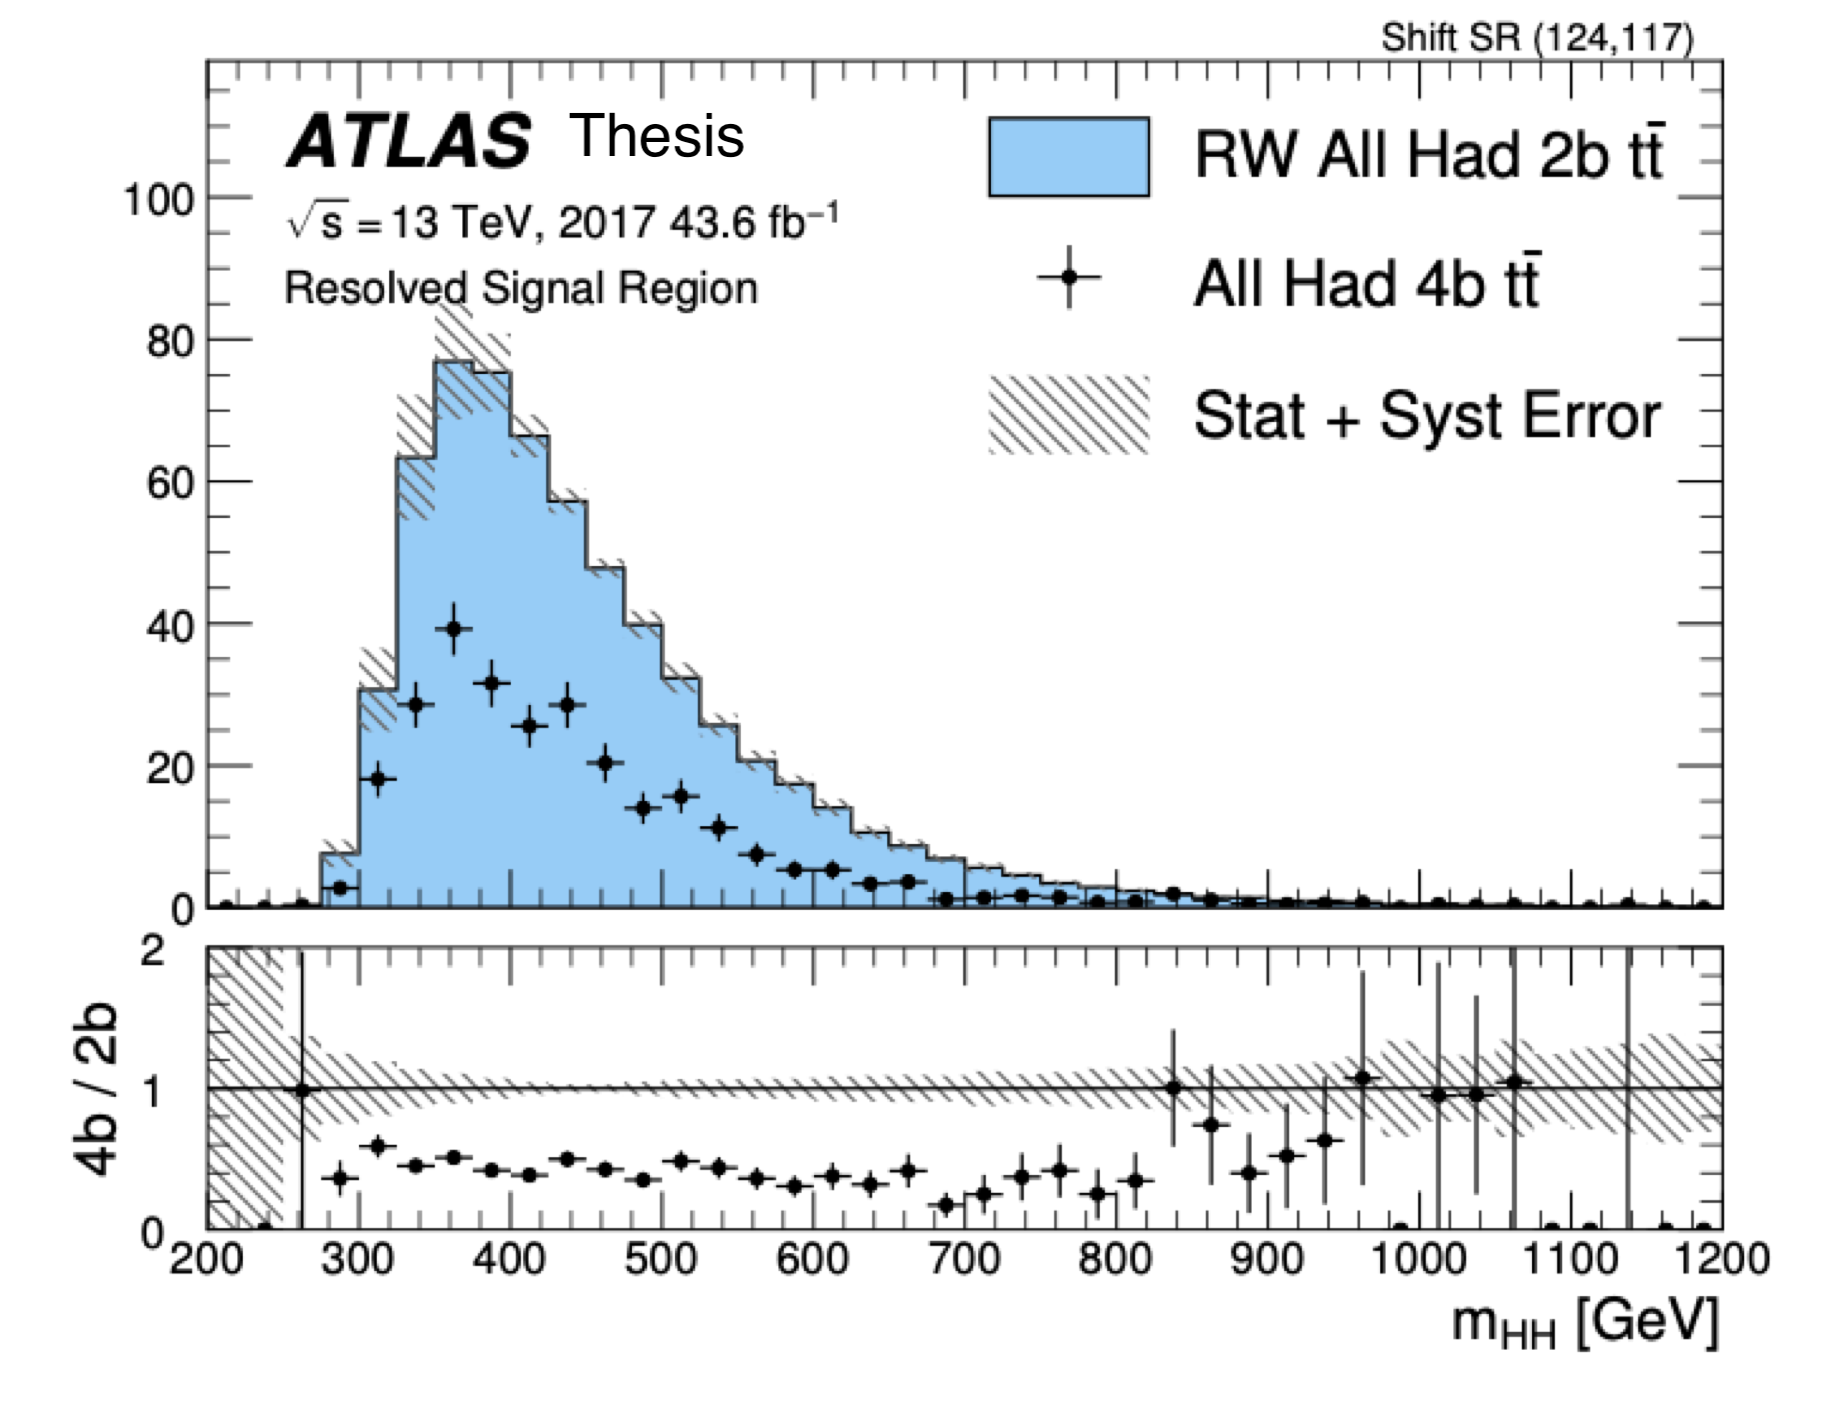
\includegraphics[width=.44\textwidth]{{figures/my_dihiggs/mHH-ah-ttbar}}
		\label{fig:mHH-ah-ttbar}
	}
	\subfloat[semi-leptonic $t\bar{t}$]{
		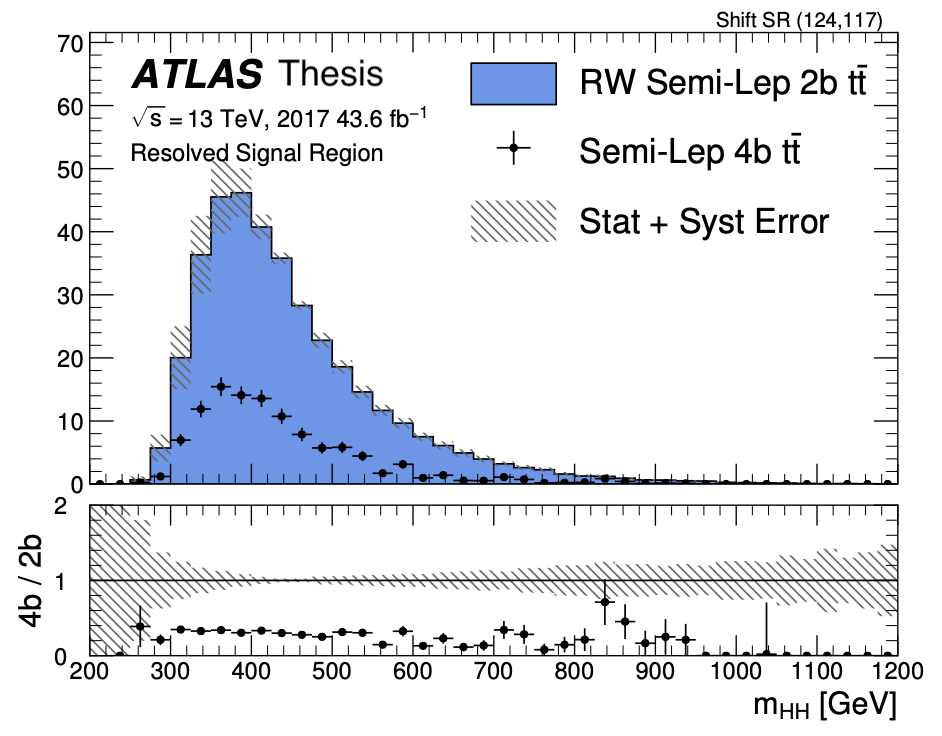
\includegraphics[width=.44\textwidth]{{figures/my_dihiggs/mHH-sl-tttbar}}
		\label{fig:mHH-sl-ttbar}
	}
	\caption{Performance of the inclusively trained reweighting evaluated on the \ttbar simulation. The performance of the inclusively trained reweighting is evaluated on 2\Pqb \ttbar simulation and compared to the 4\Pqb \ttbar prediction.
	The error bar on the background prediction shows the quadrature sum of the 2b Poisson, deep ensembles, and CR1 / CR2 shape systematic error.
	}
	\label{fig:eval-incl-ttbar-mc}
\end{figure}


\begin{itemize}
	\item Will decrease the error for negatively correlated variables
	\item Layout for this chapter
\end{itemize}

Another reason to 
Suppose that we have two random variables, $X$ and $Y$, and let $Z = X+ Y$
$\mathrm{Cov}[Z] = \mathrm{Cov}[X] + \mathrm{Cov}[Y] + 2 \mathrm{Cov}[X,Y]$

\begin{figure}[hbt]
	\centering
	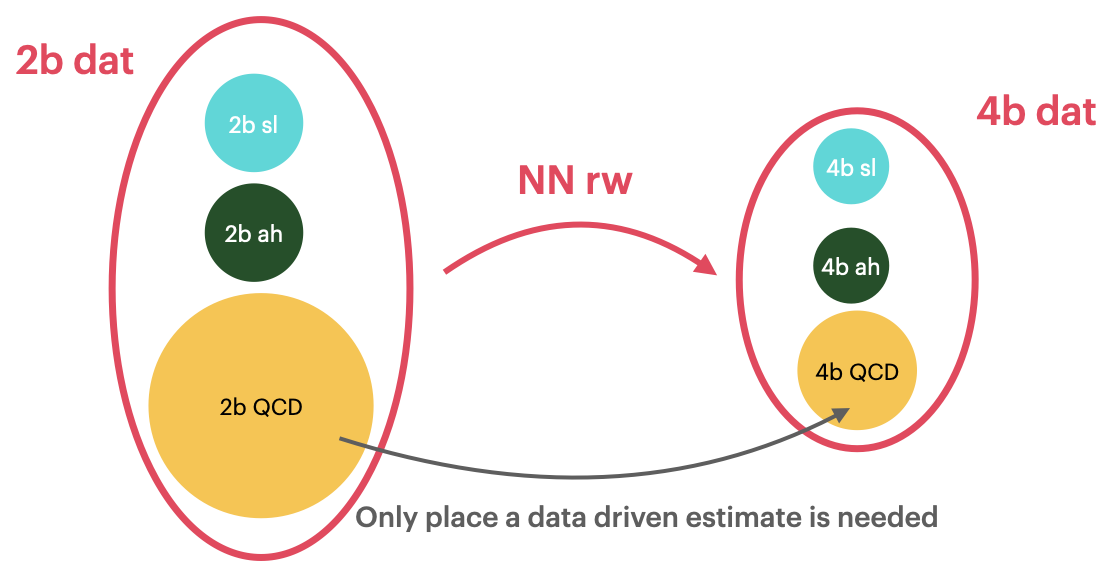
\includegraphics[width=.8\textwidth]{{figures/my_dihiggs/ttbar-rw-graphic}}
	\caption{Illustration of what how inclusively reweighting is doing to the separate components of the background estimate. The only background component that we need to use a data driven technique for is the QCD piece where we don't trust our simulation.}
	\label{fig:ttbar-rw-graphic}
\end{figure}

\section{Fitting $t\bar{t}$ templates}
\label{sec:ttbar-fits}

\subsection{Prescription}

Follows closely from the 36 \ifb analysis \cite{4b-36ifb}.

First we subtract off the 2b \ttbar from the data to get the \ttbar piece.

\begin{equation}
\textcolor{hh:darkpink}{QCD} = NN(2b dat) - NN(2b all-had t\bar{t}) - \textcolor{red}{\alpha^{sl}_{t\bar{t},2b}} \cdot NN( \textcolor{hh:lightturquoise}{2b semi-lep t\bar{t}})
\end{equation} 


\begin{equation*}
\textcolor{red}{QCD} = \frac{}{}
\end{equation*} 


\begin{figure}
\centering
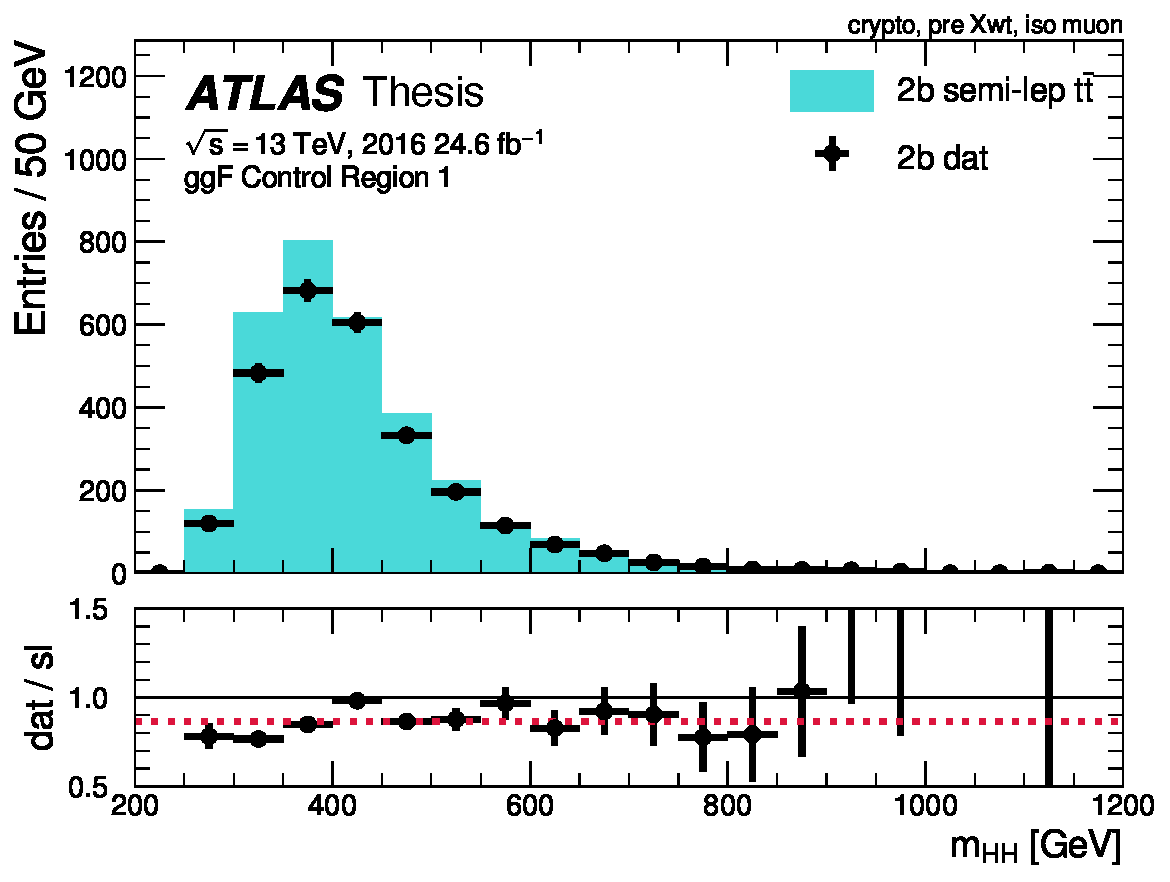
\includegraphics[width=.6\textwidth]{figures/ttbar-rw/Q45/alpha2b_control_rw_to_4b_sf.pdf}
\caption{\mhh in 2\Pqb sample with an isolated muon for 2016 data in CR1. The dashed red line in the subpanel shows the fitted $ \alpha^{sl}_{t\bar{t},2b}$}
\label{fig:alpha-2b-sl}
\end{figure}

\begin{table}[h]
	\centering
	\setlength\extrarowheight{5pt}
	\begin{tabular}{c|c|c|c}
	{SF} & {16} & {17} & {18}  \\
	\hline
	CR1 & $0.86$ & $0.80$ &  $0.83$ \\
	CR2 & $0.82$ & $0.81$ &  $0.79$ \\
	\end{tabular}
	\caption{Fitted SFs for $ \alpha^{sl}_{t\bar{t},2b}$.}
	\label{tab:pure-qcd-fits}
\end{table}


Since we will fit the \Xwt histogram to extract the template normalizations, here the networks are trained in CR1 \emph{before} applying the \Xwt $>$ 1.5 cut.

Then the next step is to do a combined fit for 4b considering top sensitive control regions:
\begin{itemize}
	\item 4b data that includes and isolated $\mu$ (helps pin-down the semi-lep \ttbar component)
	\item An \Xwt shape fit (helps discriminate between the all-had \ttbar and qcd templates).
\end{itemize}

\begin{figure}
\centering
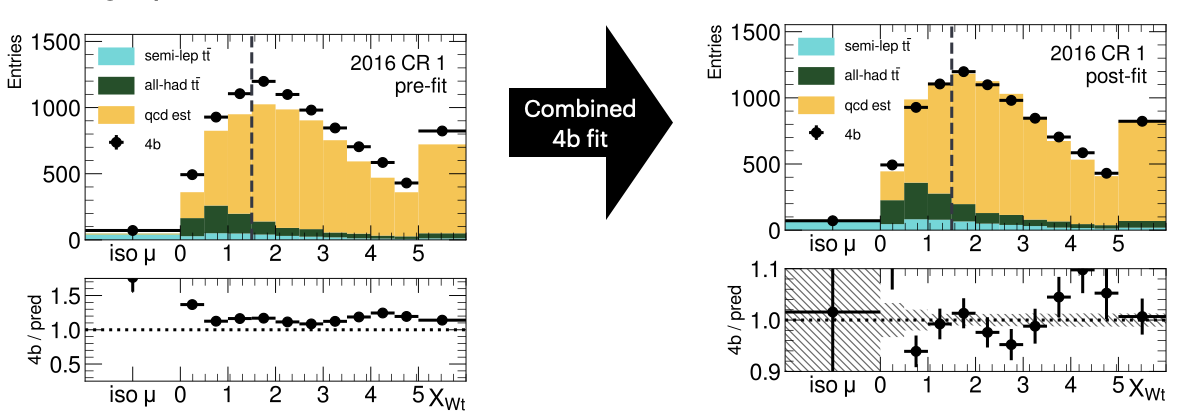
\includegraphics[width=.8\textwidth]{{figures/my_dihiggs/ttbar-pre-post-comb-fit}}
\caption{CR1 fits}
%\label{fig:alpha-2b-sl}
\end{figure}

\subsection{Fit results 4b}

\begin{figure}
\centering
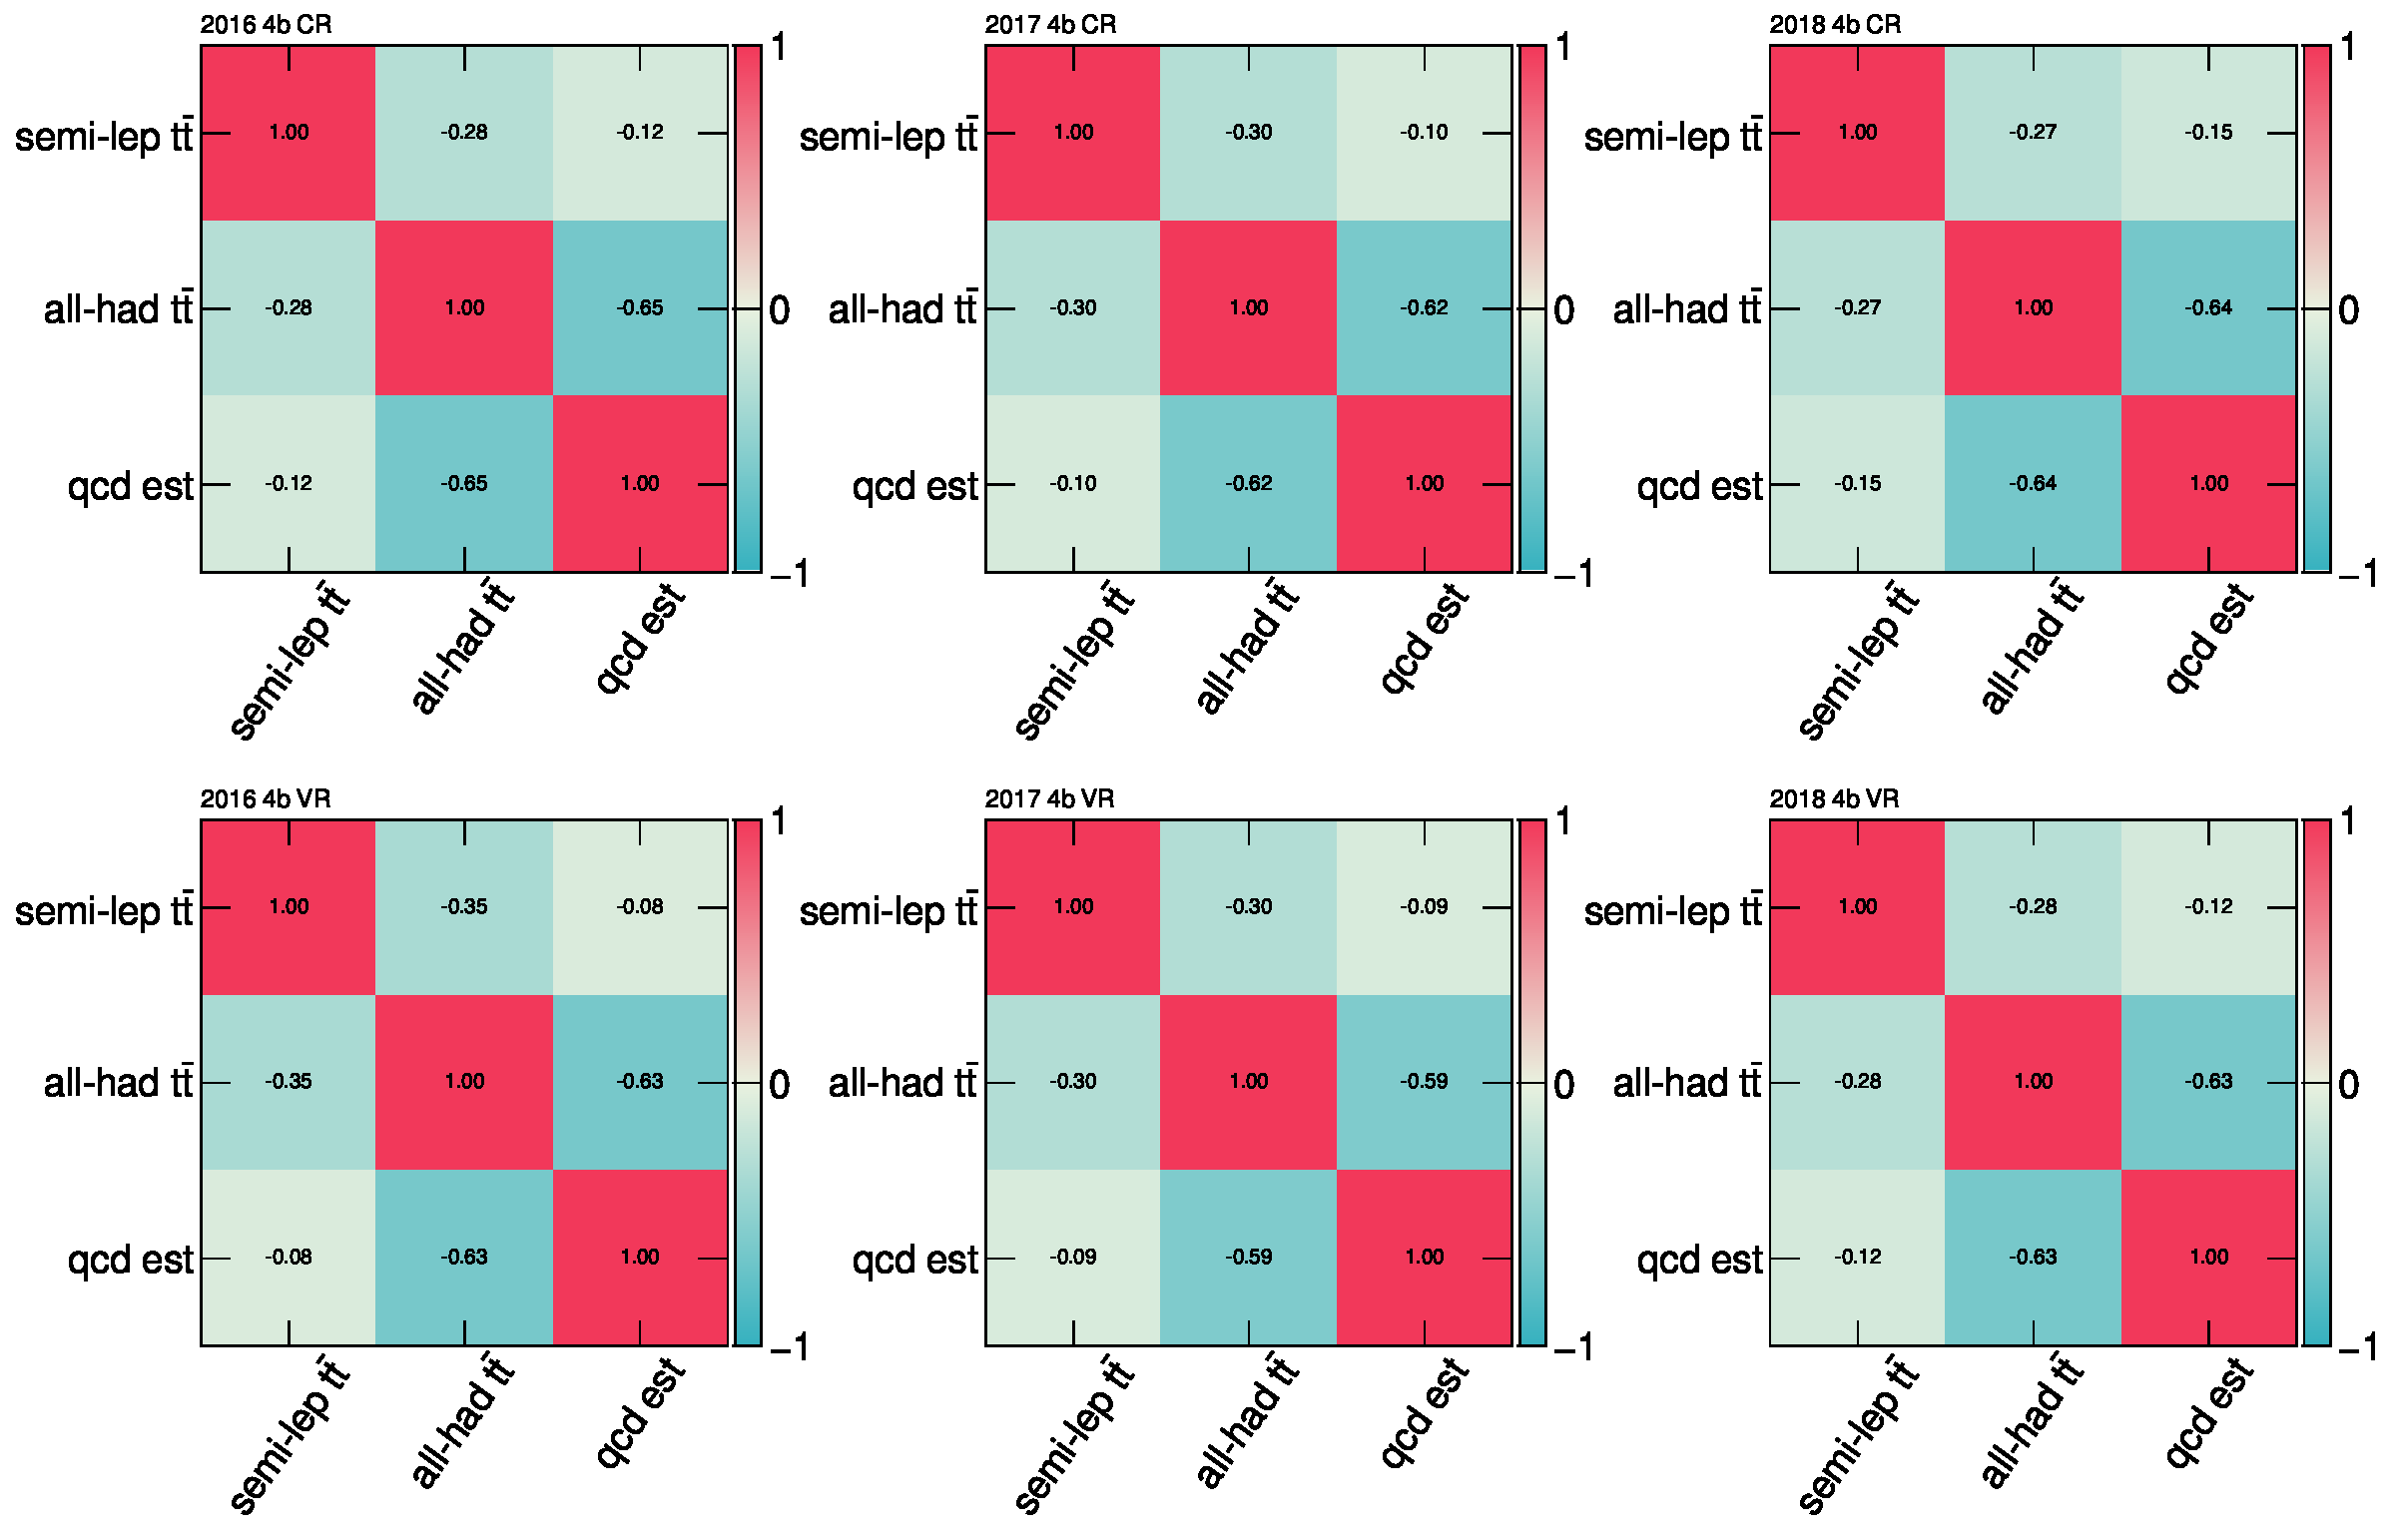
\includegraphics[width=\textwidth]{figures/ttbar-rw/Q45/fitCorr-4b-CR-VR-16-17-18_3compFits.pdf}
\caption{CR1 fits}
%\label{fig:alpha-2b-sl}
\end{figure}

\begin{figure}
\centering
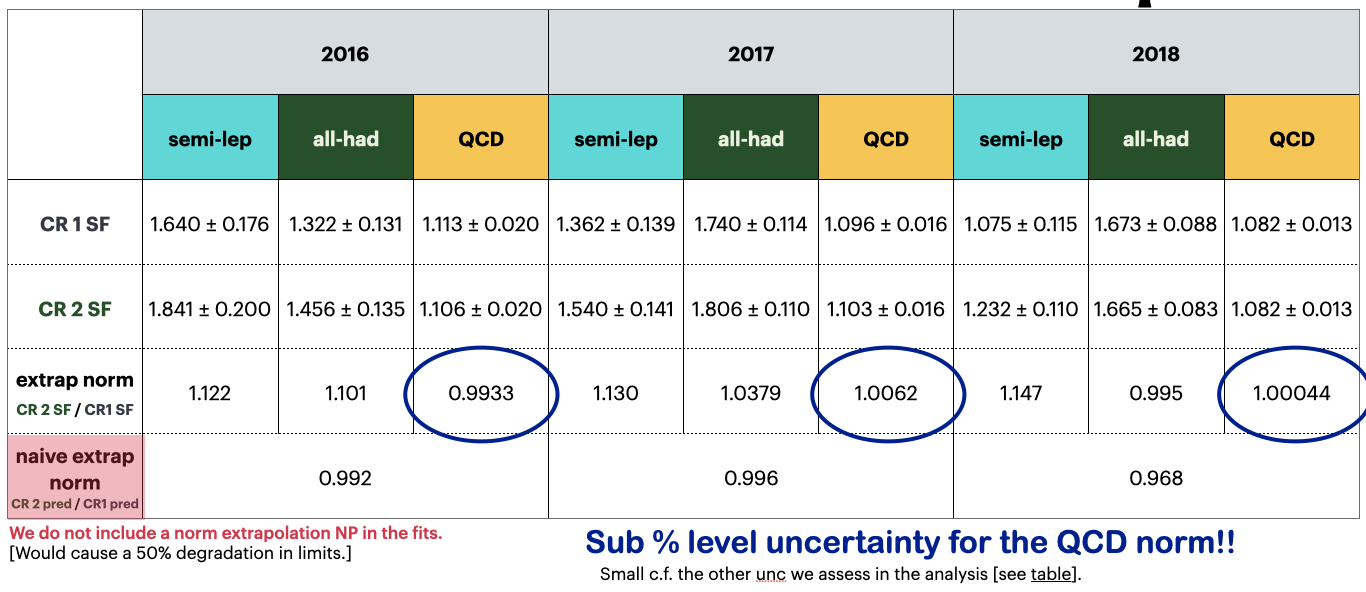
\includegraphics[width=.8\textwidth]{{figures/my_dihiggs/sfs-4b-ttbar-fits}}
\caption{}
%\label{fig:alpha-2b-sl}
\end{figure}

\begin{figure}
\centering
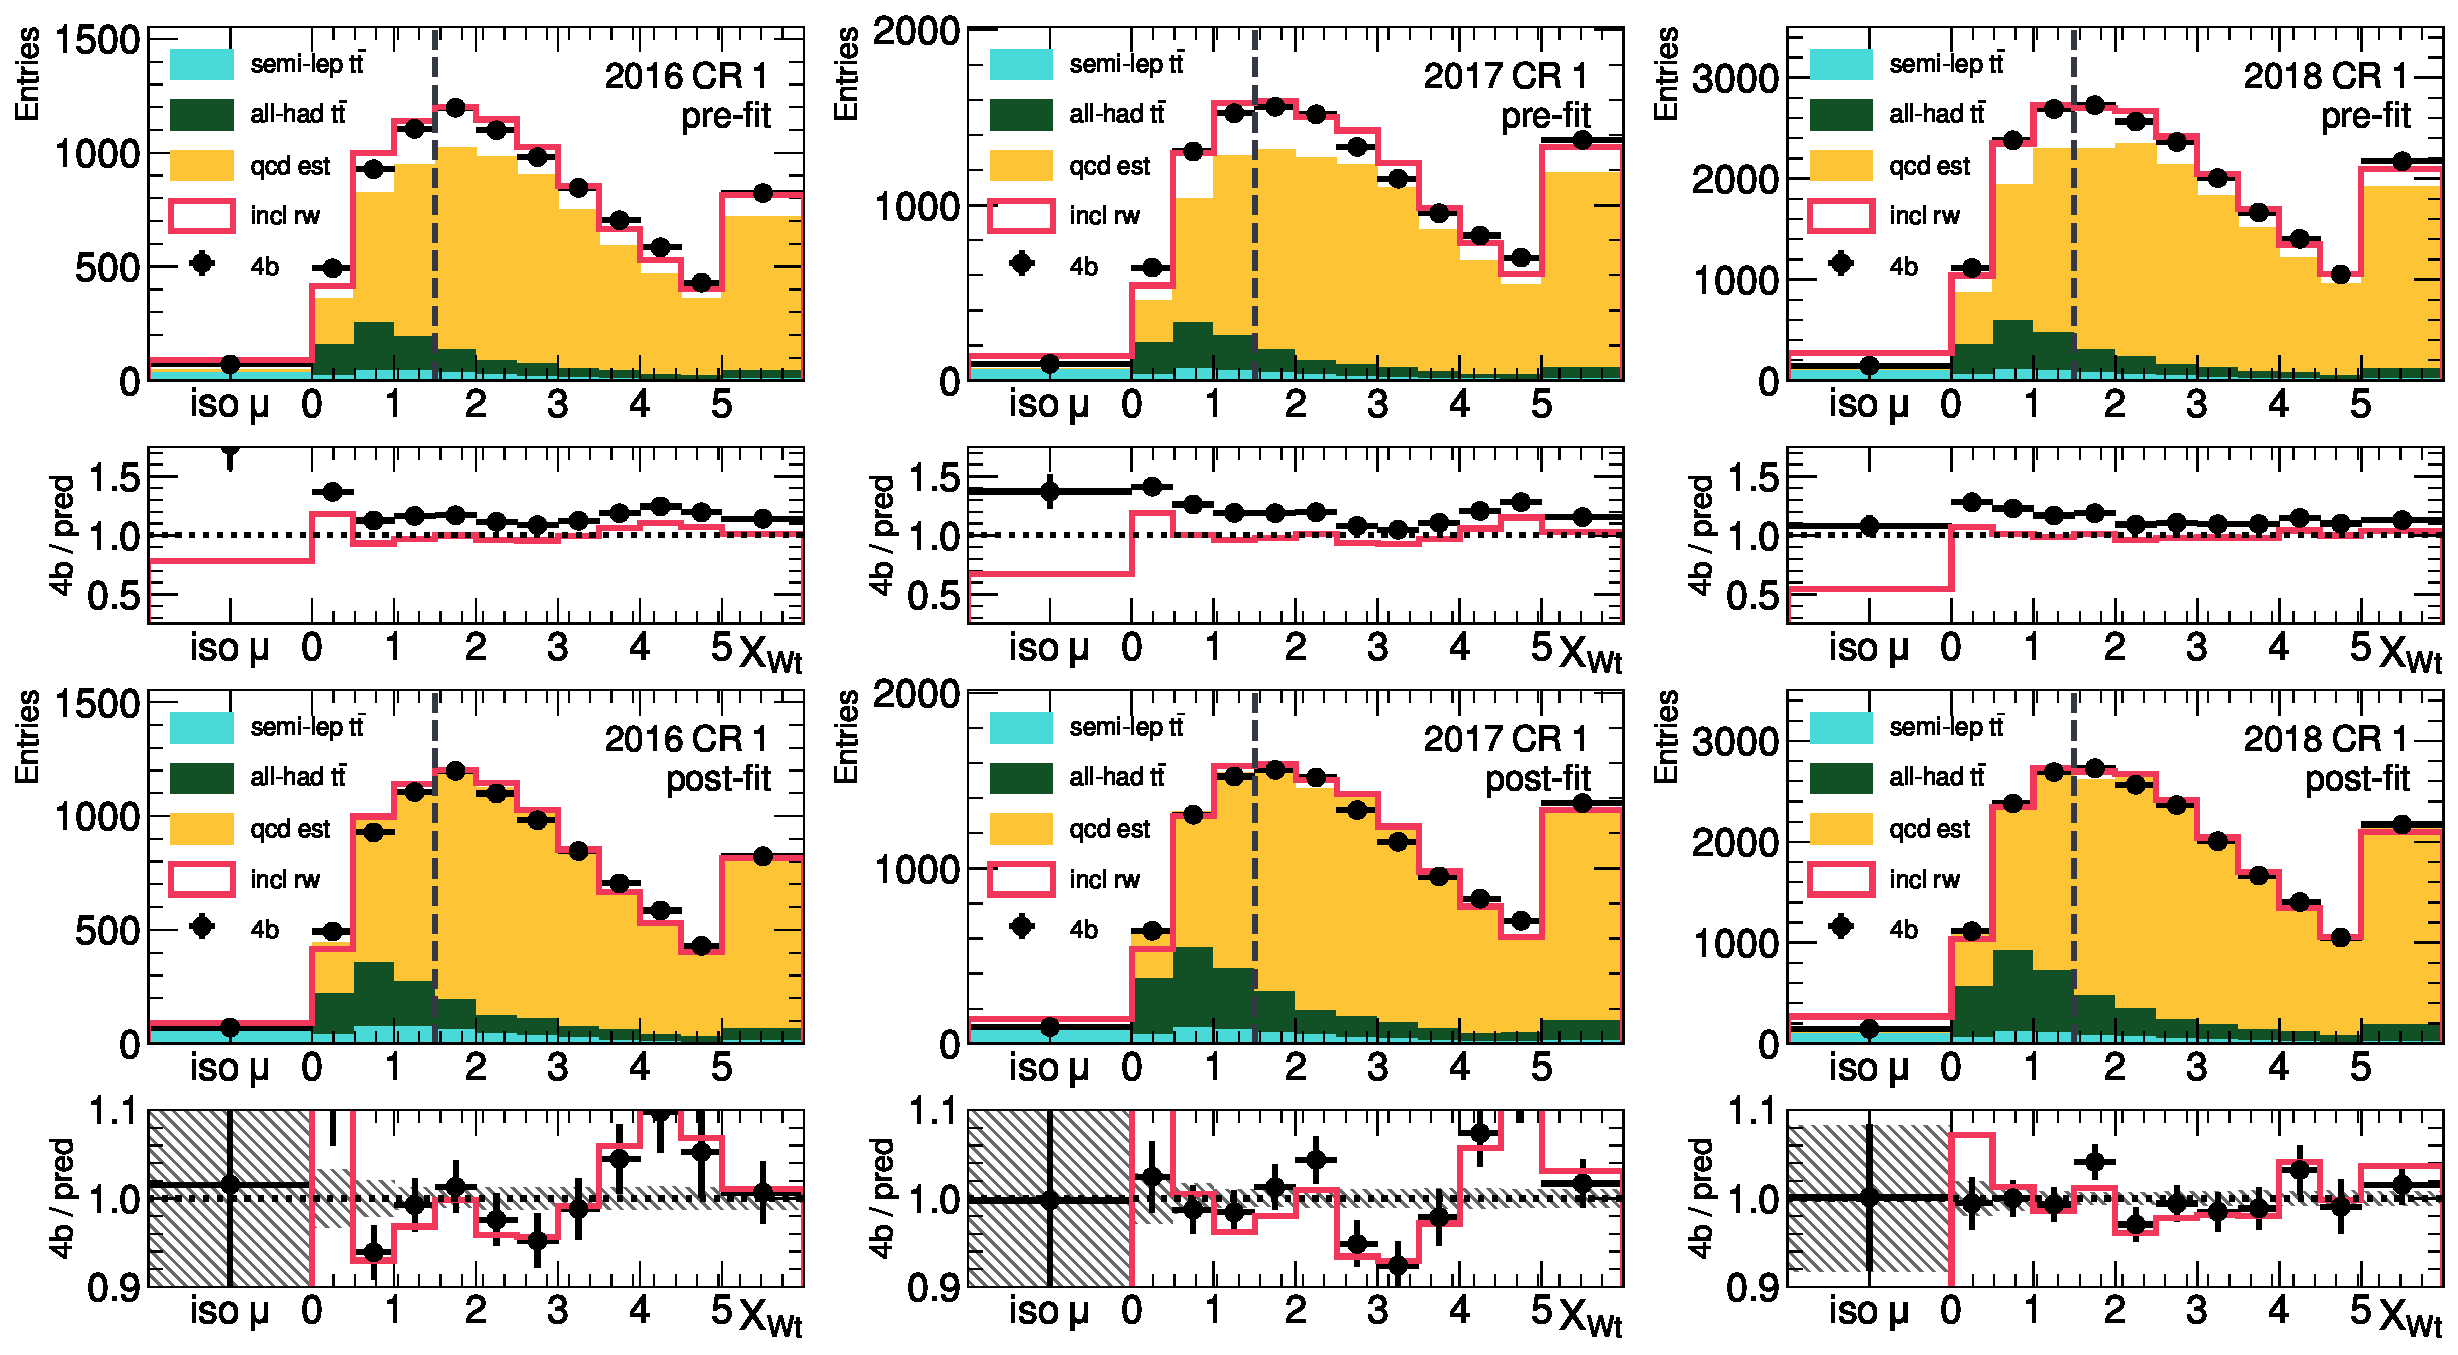
\includegraphics[width=\textwidth]{figures/ttbar-rw/Q45/prePostFit-CR1-16-17-18_4b_12_Xwt_bins_3compFits_rw.pdf}
\caption{CR1 fit in CR1}
%\label{fig:alpha-2b-sl}
\end{figure}

Next, we look at a few variables after the \Xwt $>$ 1.5 cut.

\begin{figure}
\centering
\subfloat[2016]{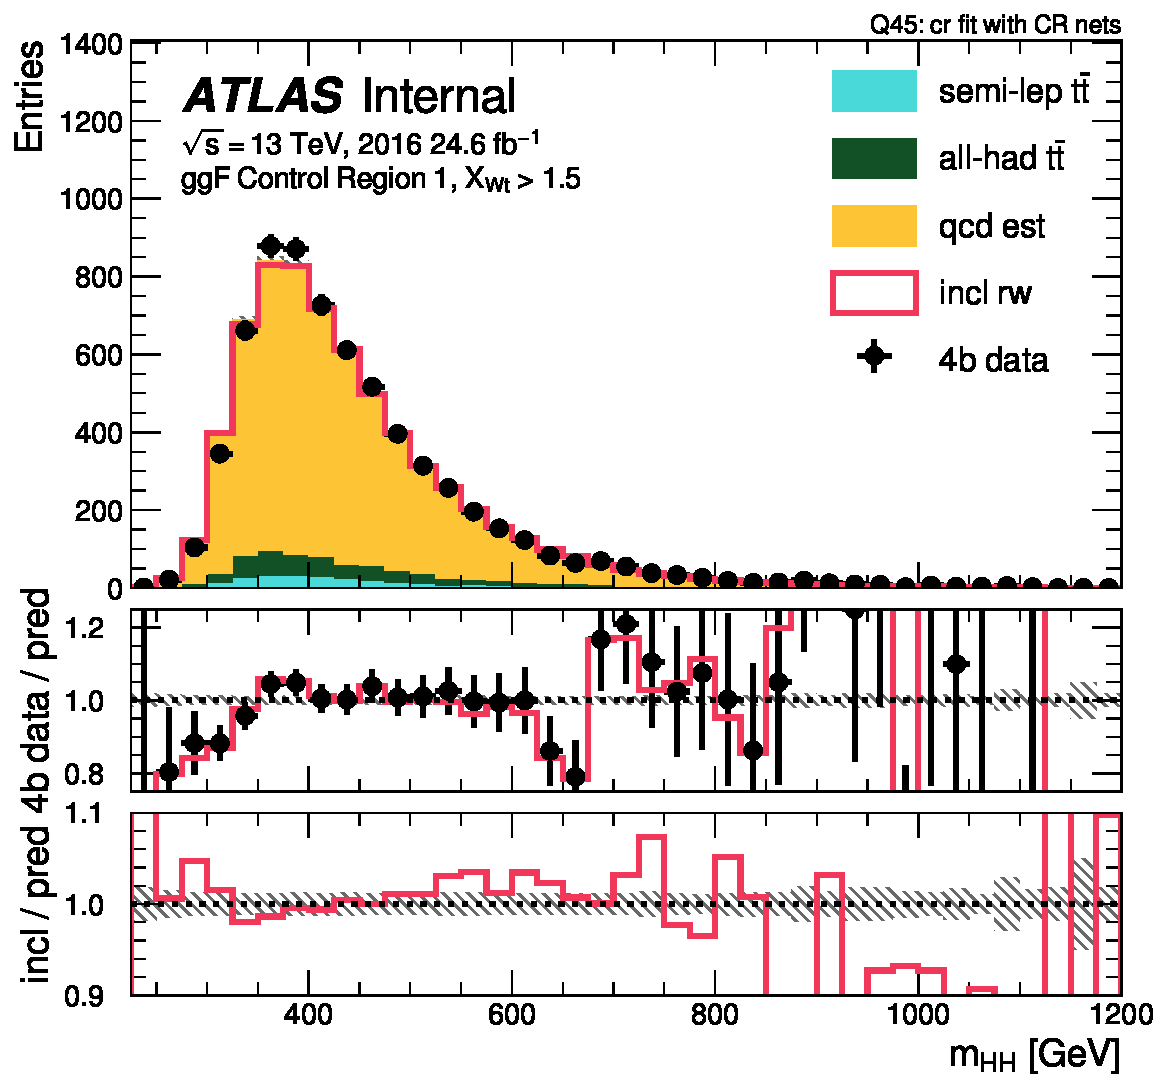
\includegraphics[width=.33\textwidth]{{figures/ttbar-rw/Q45/crFit_Xwtcut_1.5/m_hh_4b_CR1_16}}}
\subfloat[2017]{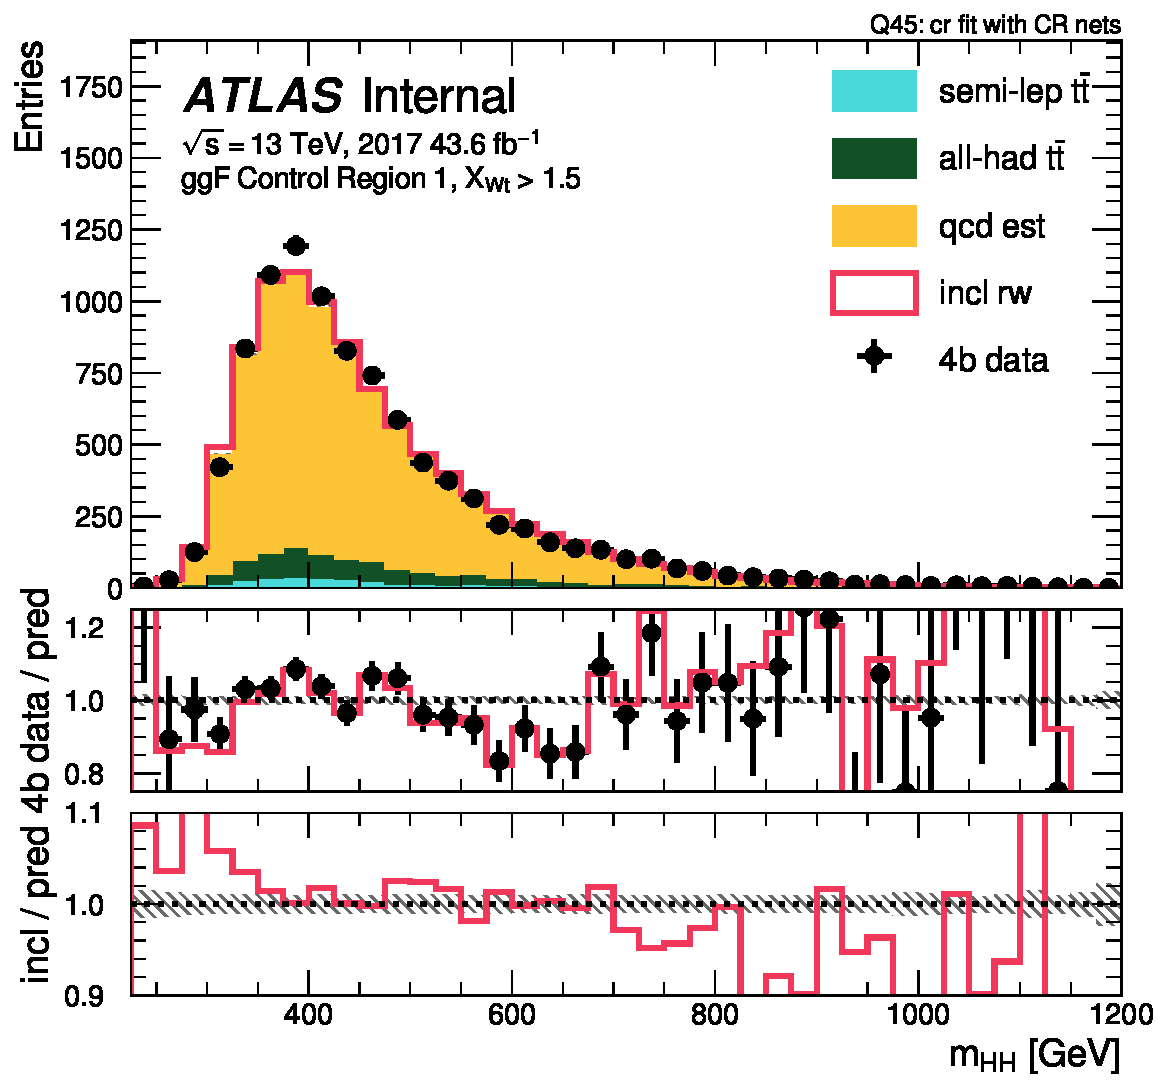
\includegraphics[width=.33\textwidth]{{figures/ttbar-rw/Q45/crFit_Xwtcut_1.5/m_hh_4b_CR1_17}}}
\subfloat[2018]{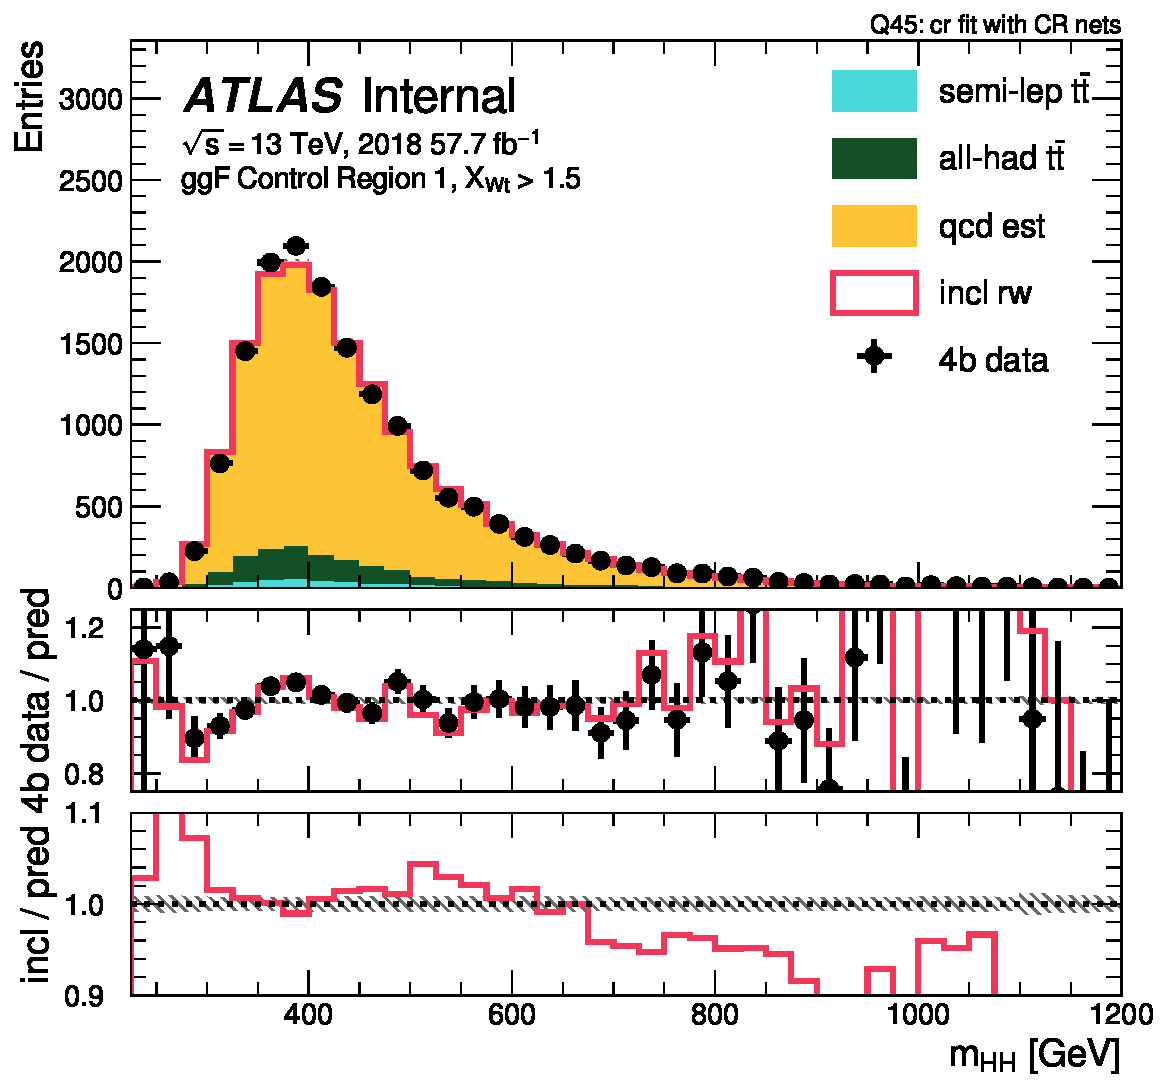
\includegraphics[width=.33\textwidth]{{figures/ttbar-rw/Q45/crFit_Xwtcut_1.5/m_hh_4b_CR1_18}}}
\caption{CR1 evaluation using the CR1 fits}
\label{fig:mhh-cr1-4b}
\end{figure}


\begin{figure}
\centering
\subfloat[2016]{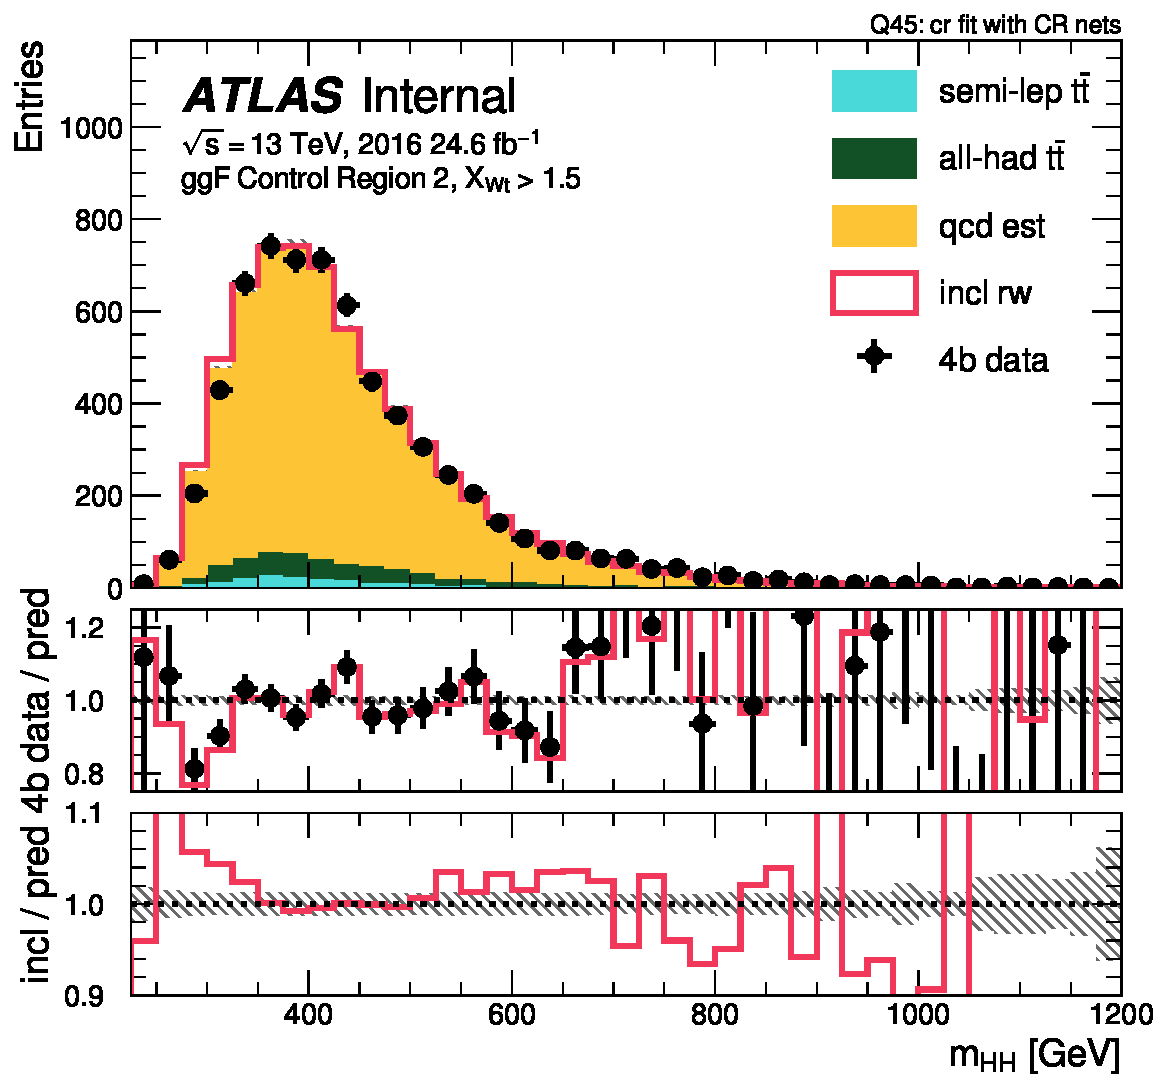
\includegraphics[width=.33\textwidth]{{figures/ttbar-rw/Q45/crFit_Xwtcut_1.5/m_hh_4b_CR2_16}}}
\subfloat[2017]{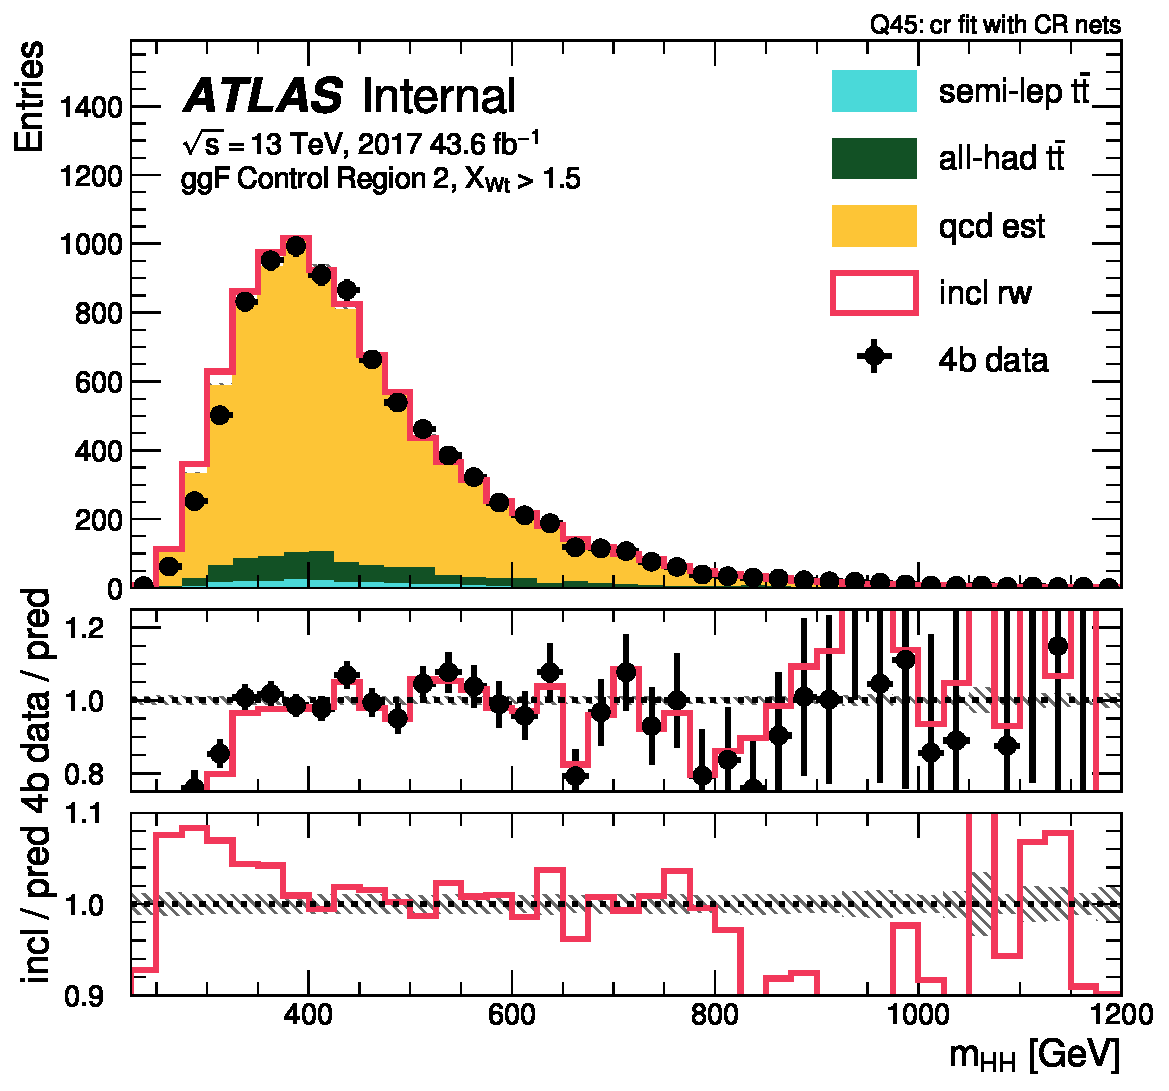
\includegraphics[width=.33\textwidth]{{figures/ttbar-rw/Q45/crFit_Xwtcut_1.5/m_hh_4b_CR2_17}}}
\subfloat[2018]{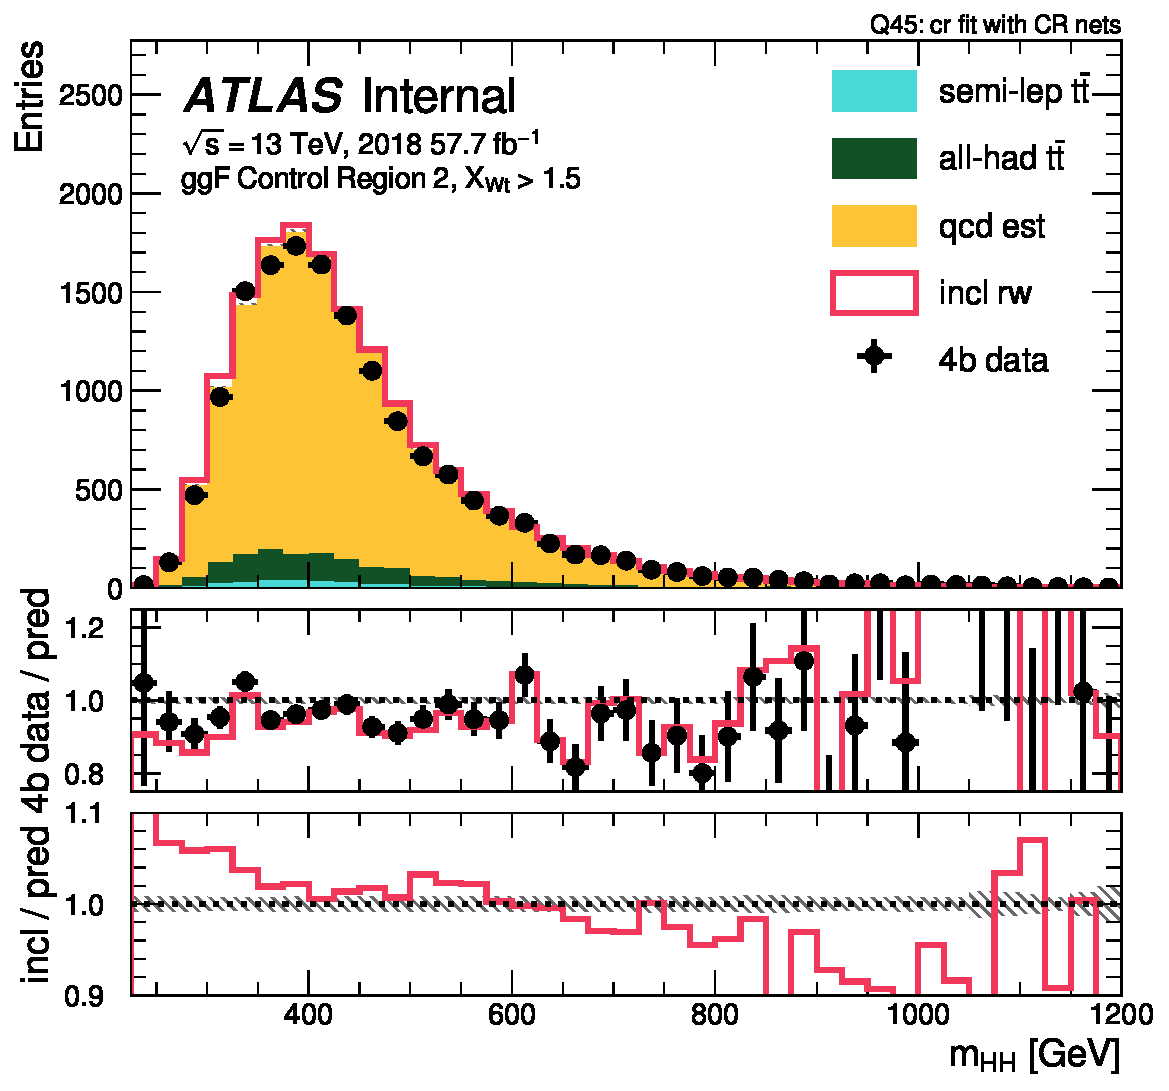
\includegraphics[width=.33\textwidth]{{figures/ttbar-rw/Q45/crFit_Xwtcut_1.5/m_hh_4b_CR2_18}}}
\caption{CR2 evaluation using the CR1 fits}
\label{fig:mhh-cr2-4b}
\end{figure}

\begin{figure}
\centering
\subfloat[2016]{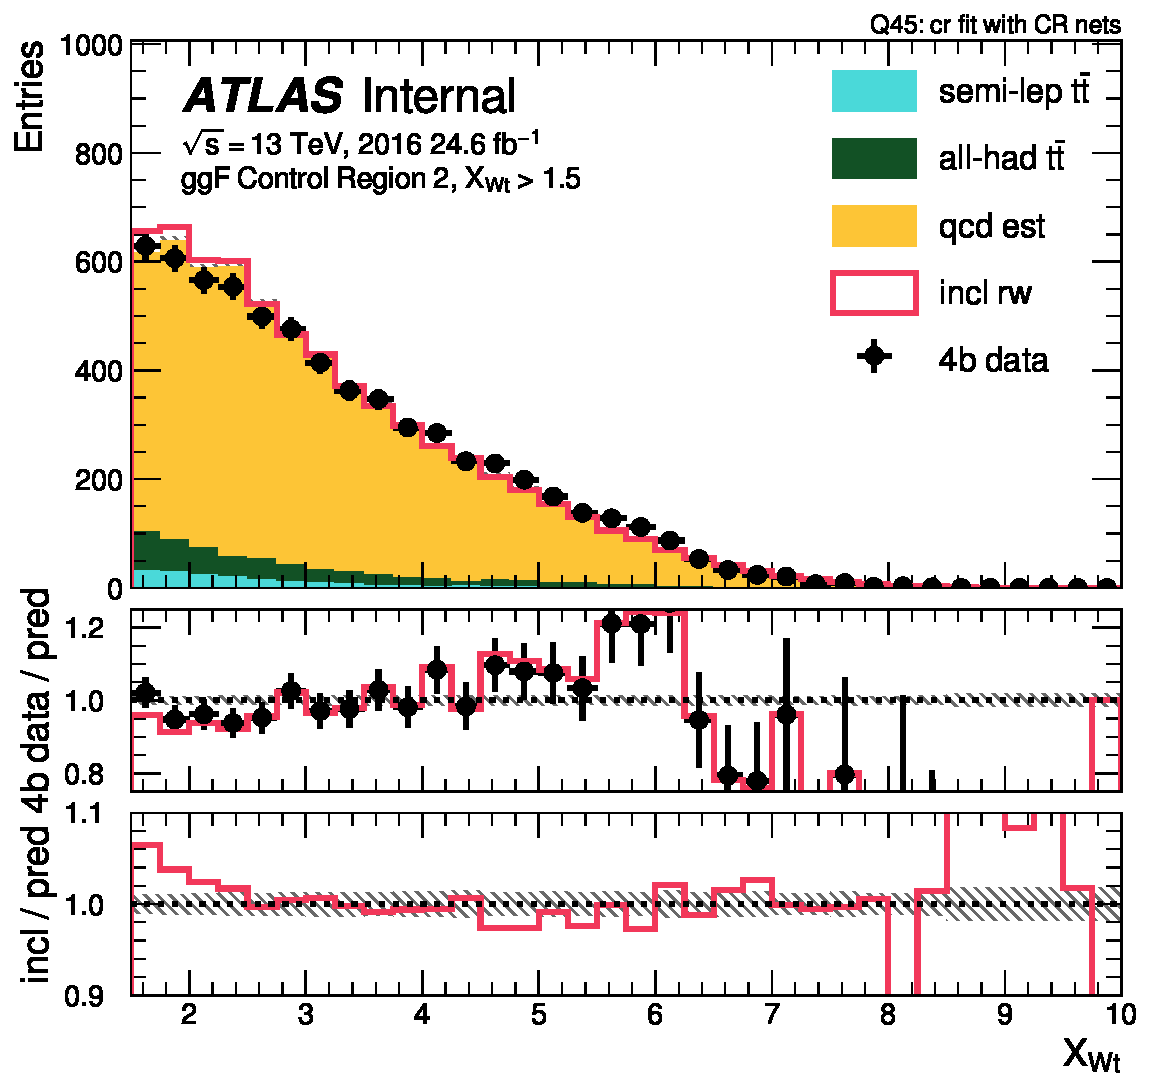
\includegraphics[width=.33\textwidth]{{figures/ttbar-rw/Q45/crFit_noXwtcut/X_wt_tag_4b_CR2_16}}}
\subfloat[2017]{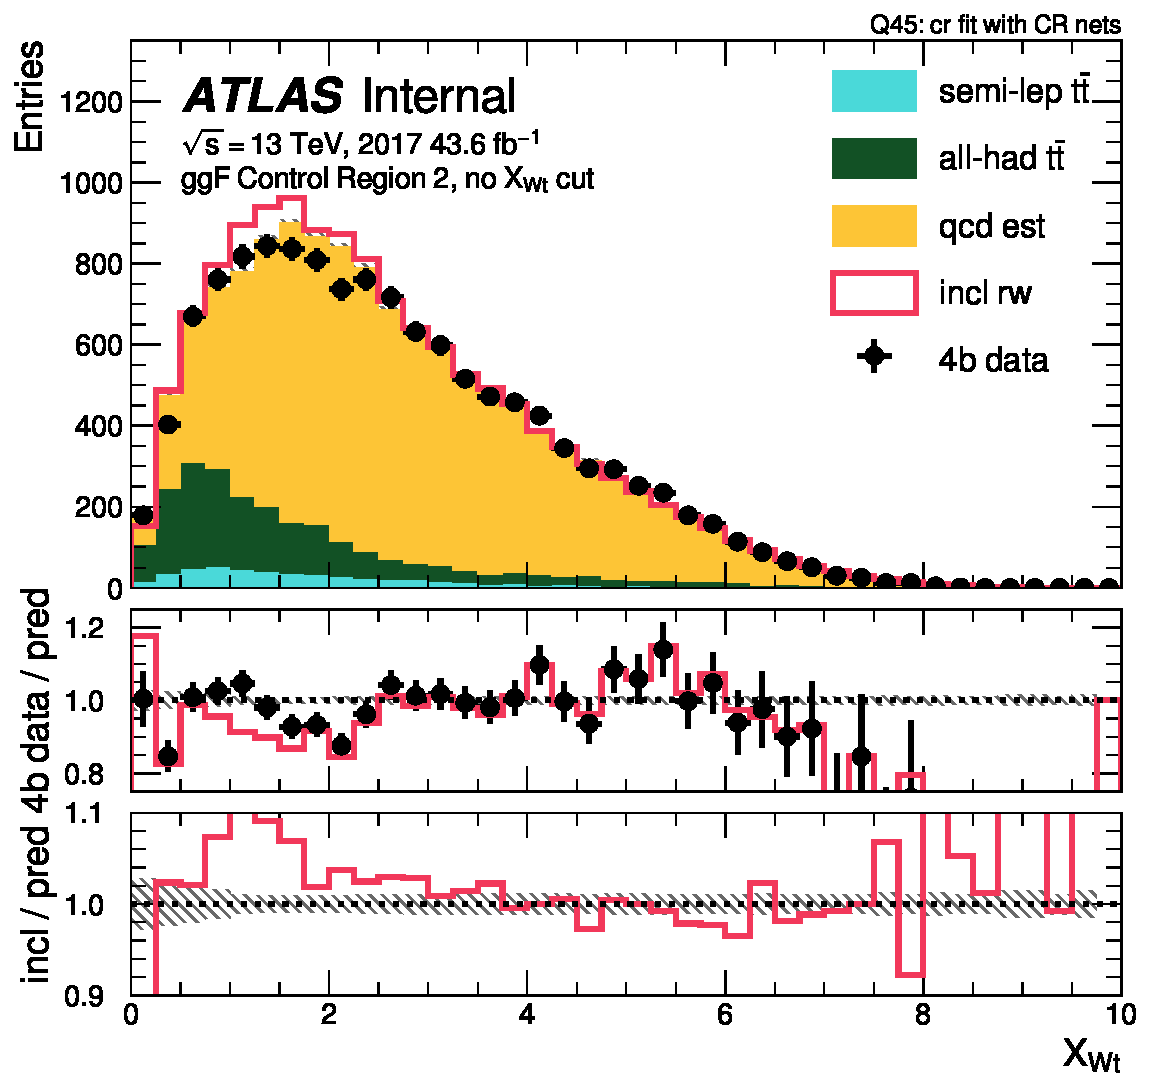
\includegraphics[width=.33\textwidth]{{figures/ttbar-rw/Q45/crFit_noXwtcut/X_wt_tag_4b_CR2_17}}}
\subfloat[2018]{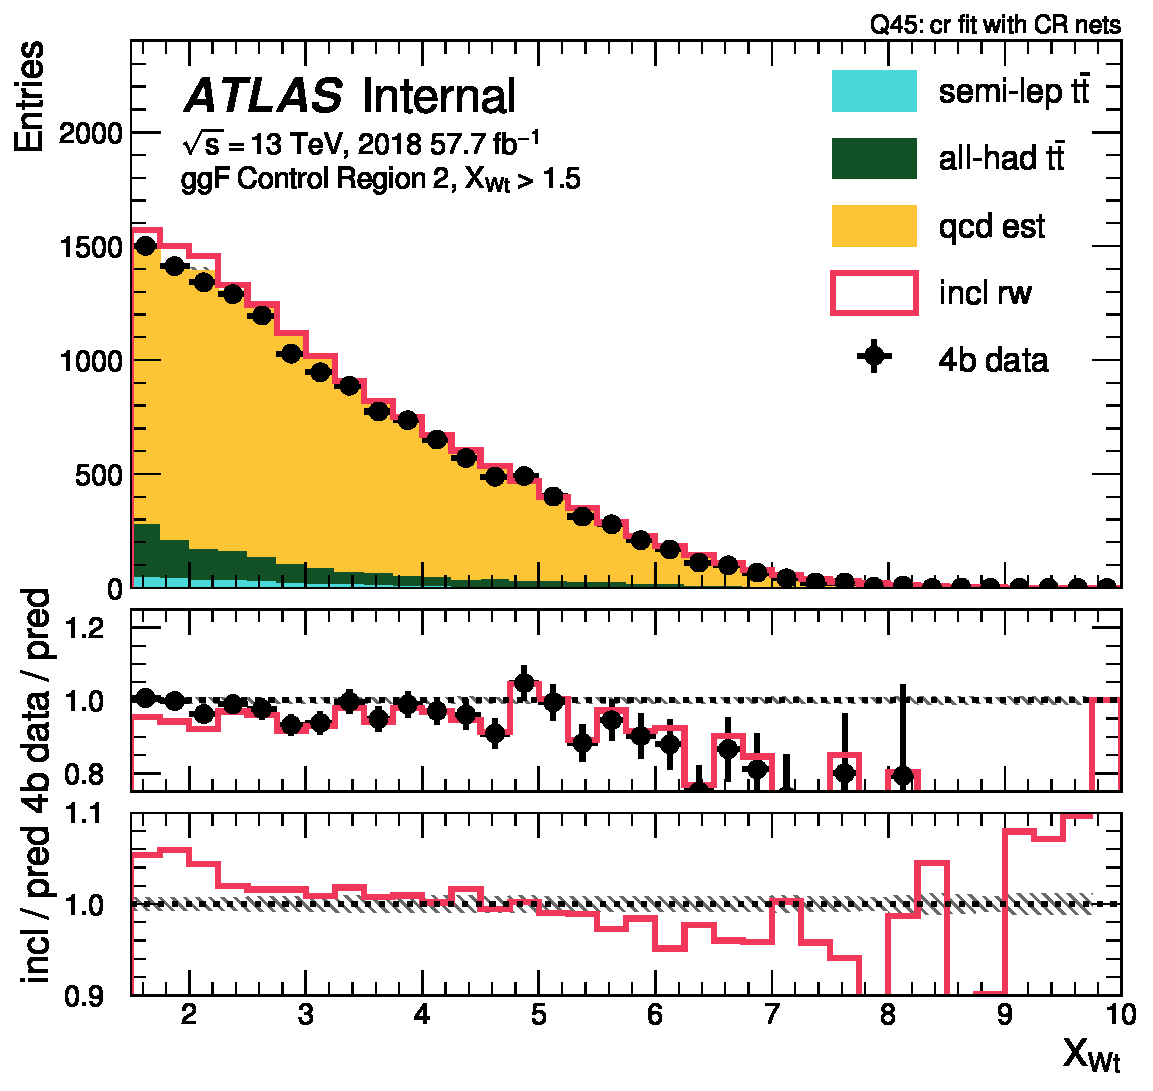
\includegraphics[width=.33\textwidth]{{figures/ttbar-rw/Q45/crFit_noXwtcut/X_wt_tag_4b_CR2_18}}}
\caption{CR2 evaluation using the CR1 fits}
\label{fig:Xwt-cr2-4b}
\end{figure}

\FloatBarrier
\clearpage
\subsection{Fit results 3b1f}

\begin{figure}[htb]
\centering
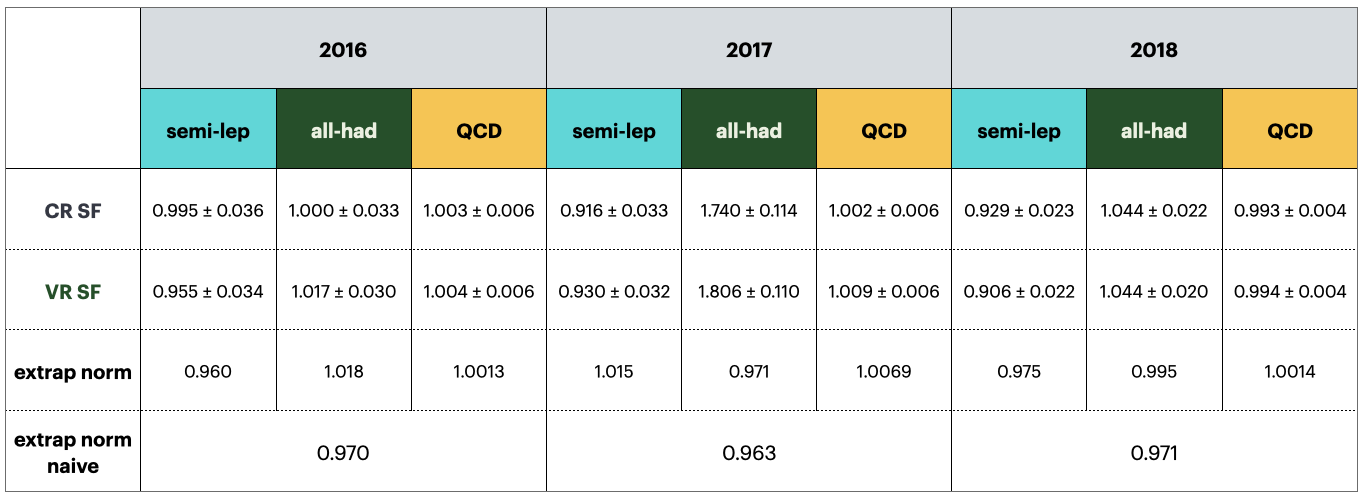
\includegraphics[width=.8\textwidth]{{figures/my_dihiggs/sfs-3b1f-ttbar-fits}}
\caption{}
\label{tab:sfs-3b1f-ttbar-fits}
\end{figure}

\begin{figure}[htb]
\centering
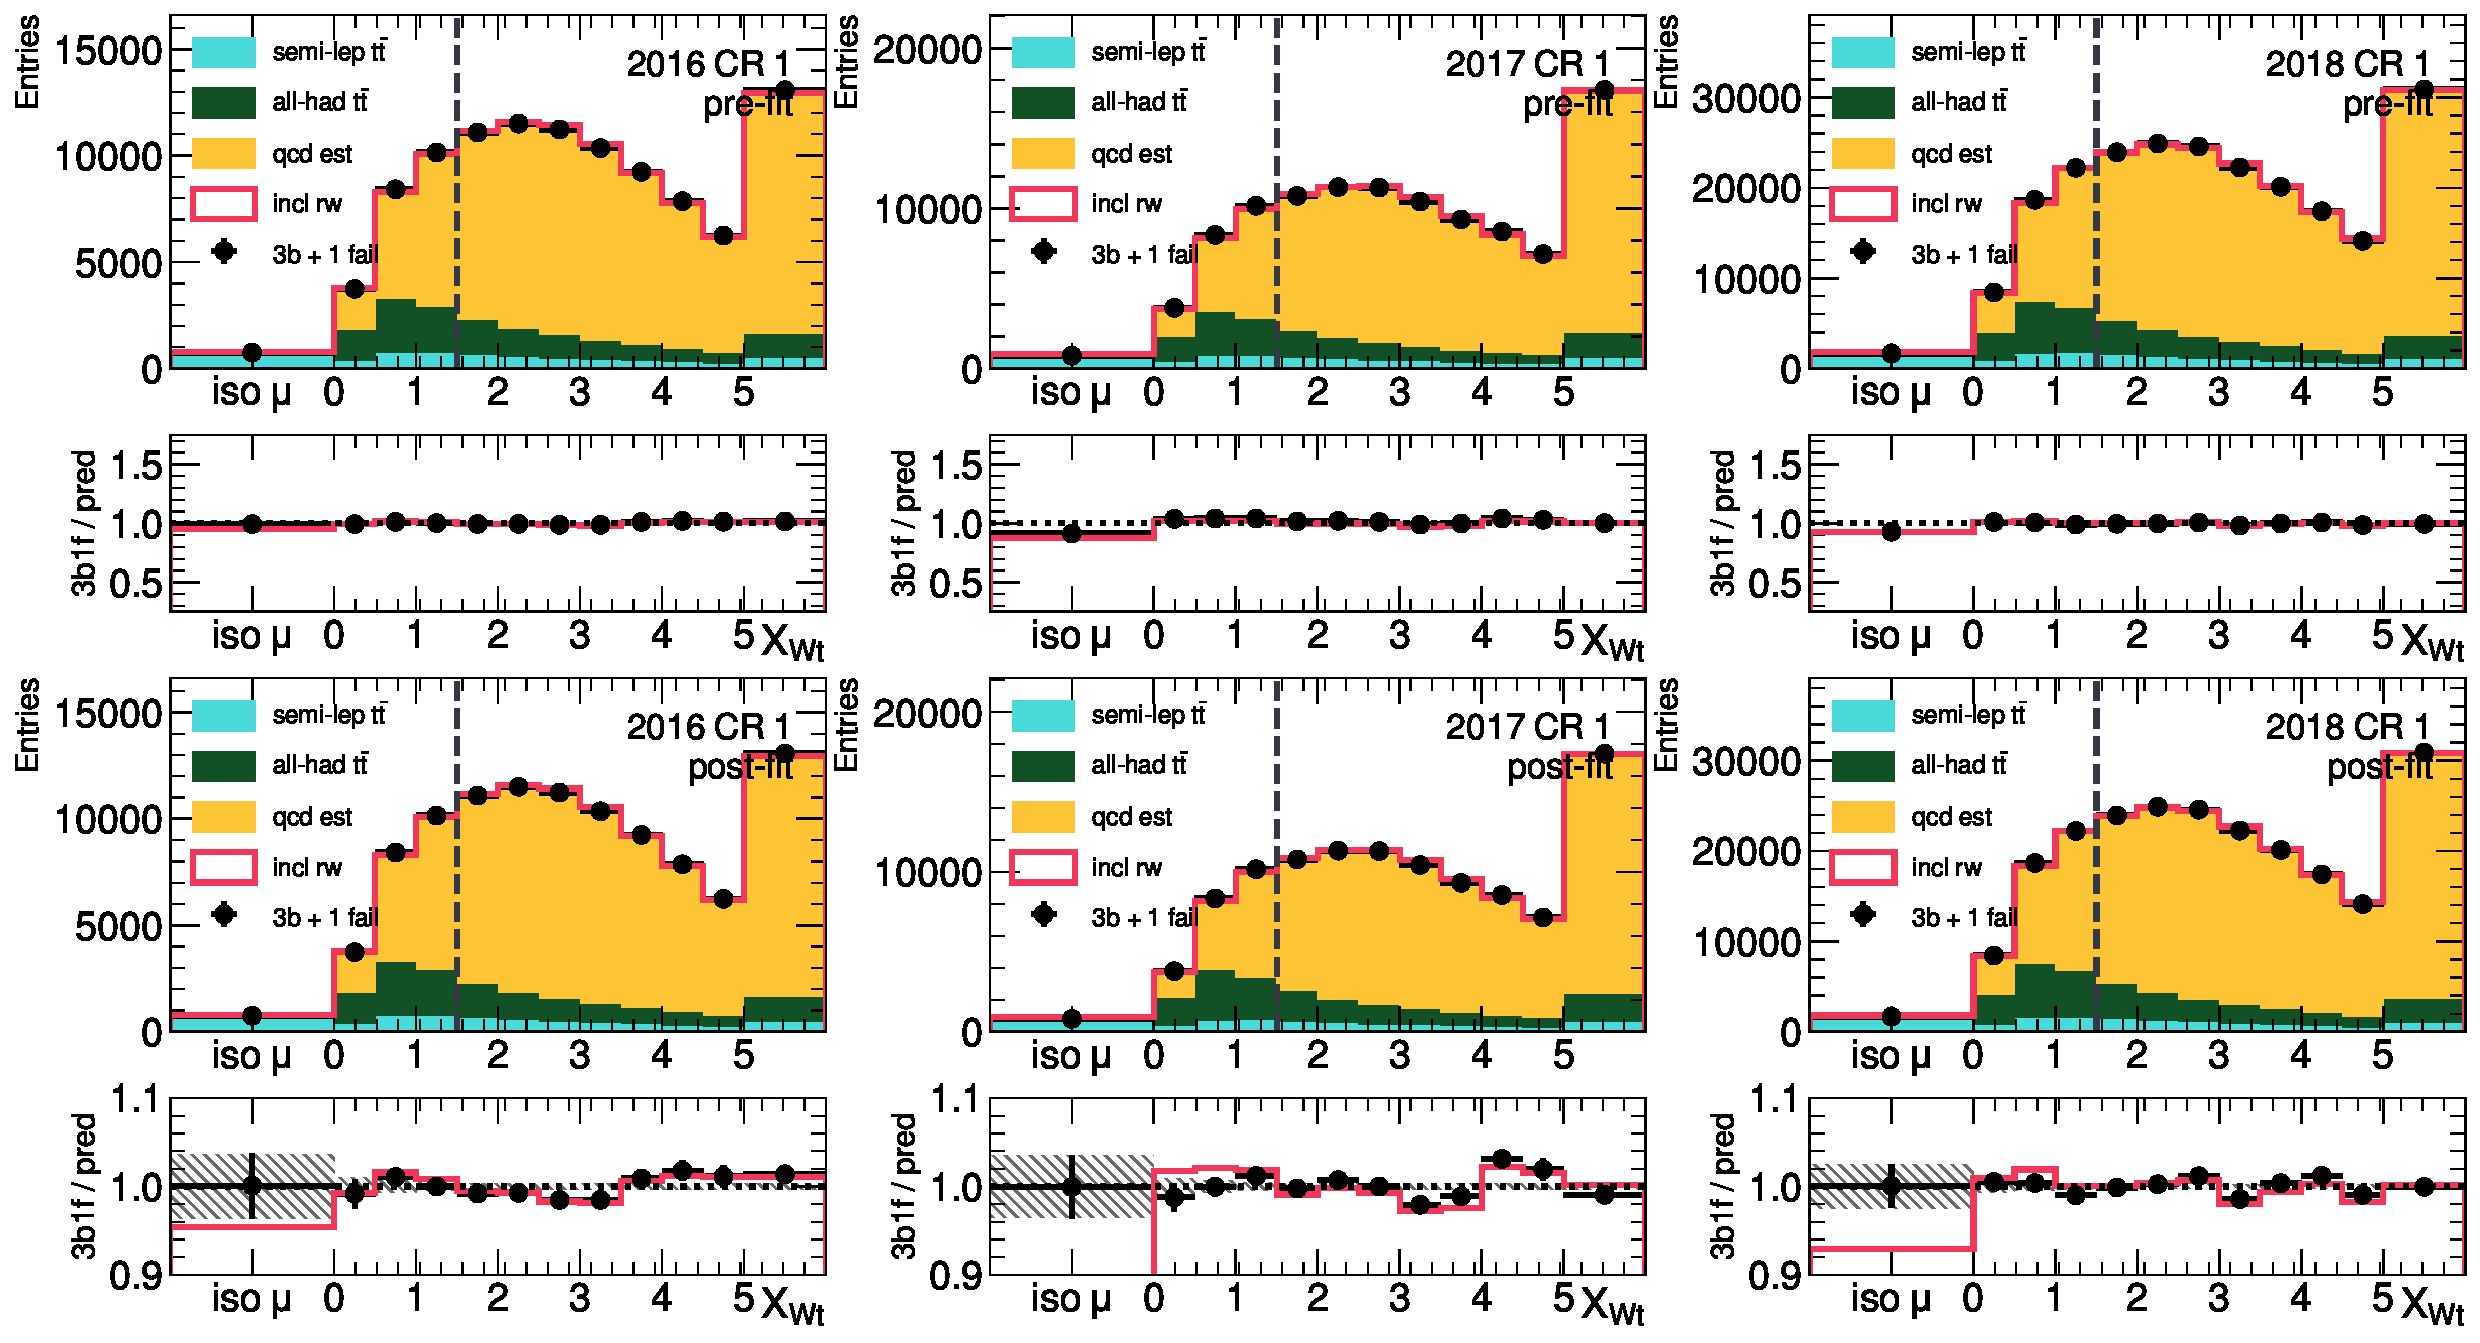
\includegraphics[width=\textwidth]{figures/ttbar-rw/Q45/prePostFit-CR1-16-17-18_3b1f_12_Xwt_bins_3compFits_rw.pdf}
\caption{CR1 fit in CR1}
%\label{fig:alpha-2b-sl}
\end{figure}


\begin{figure}
\centering
\subfloat[2016]{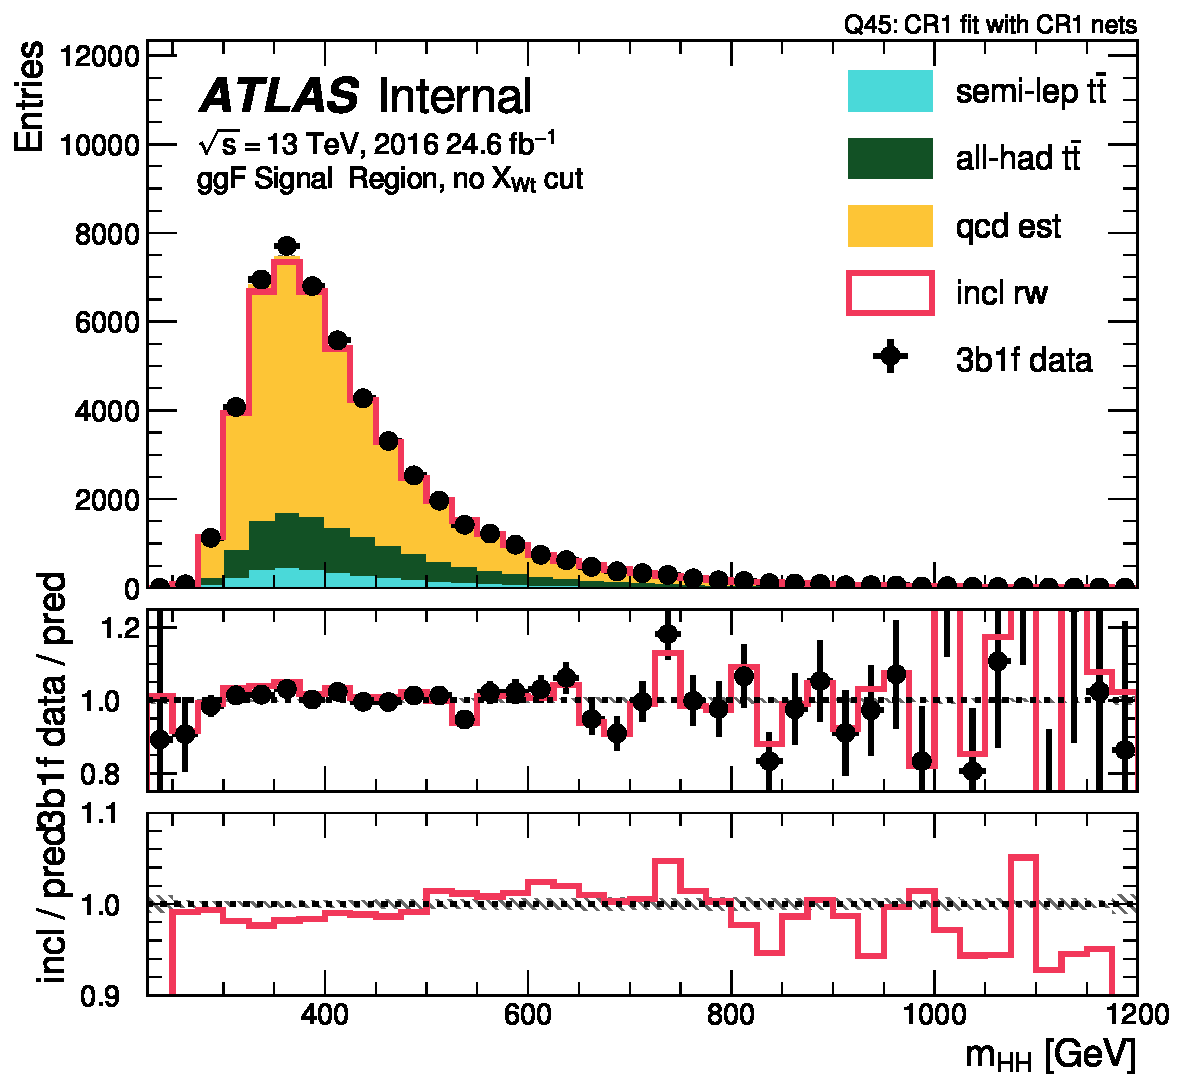
\includegraphics[width=.33\textwidth]{{figures/ttbar-rw/Q45/crFit_Xwtcut_1.5/m_hh_3b1f_SR_16}}}
\subfloat[2017]{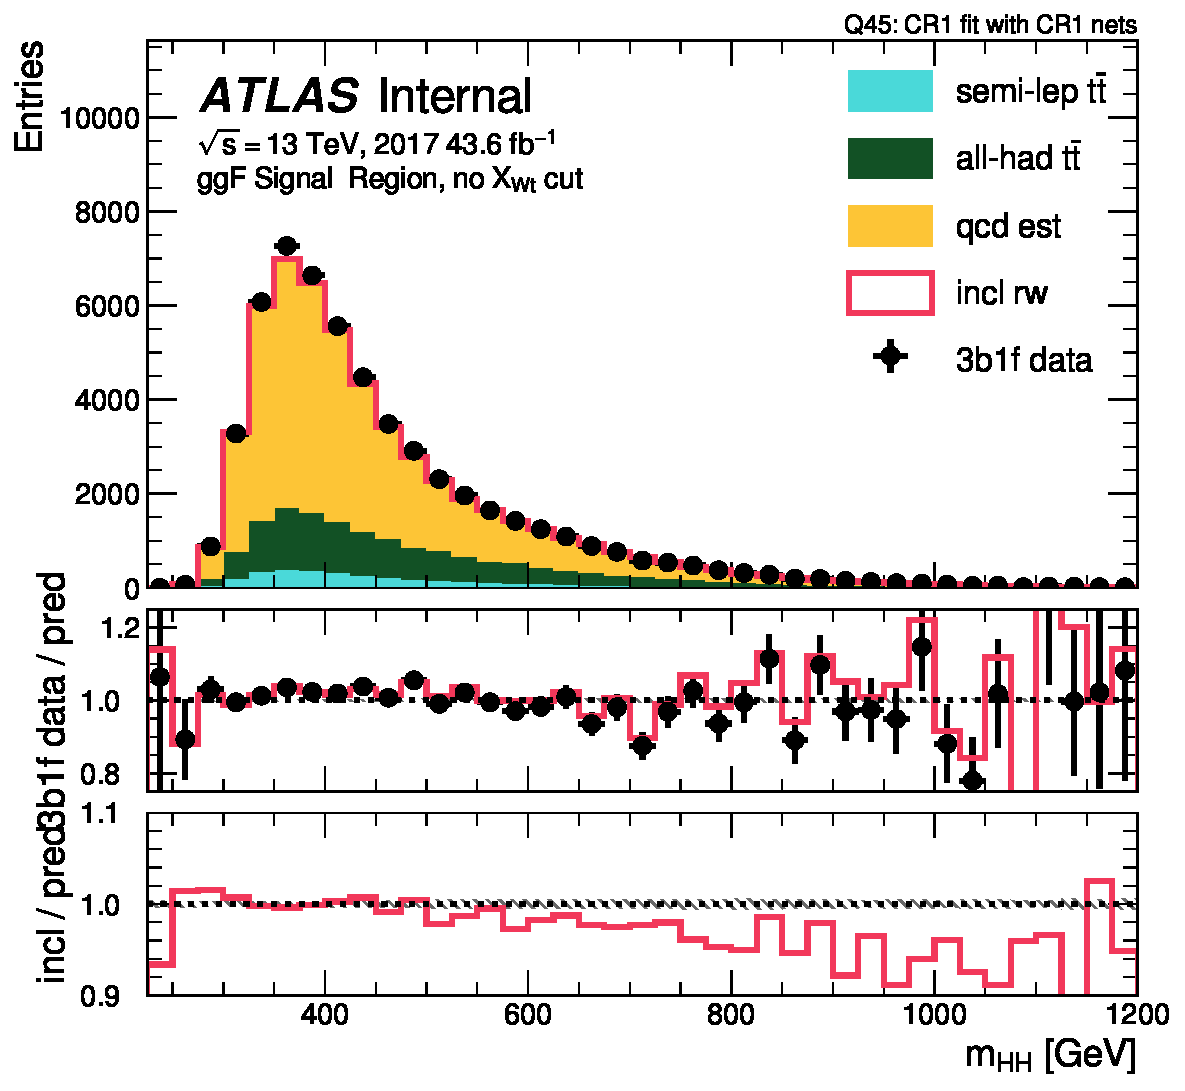
\includegraphics[width=.33\textwidth]{{figures/ttbar-rw/Q45/crFit_Xwtcut_1.5/m_hh_3b1f_SR_17}}}
\subfloat[2018]{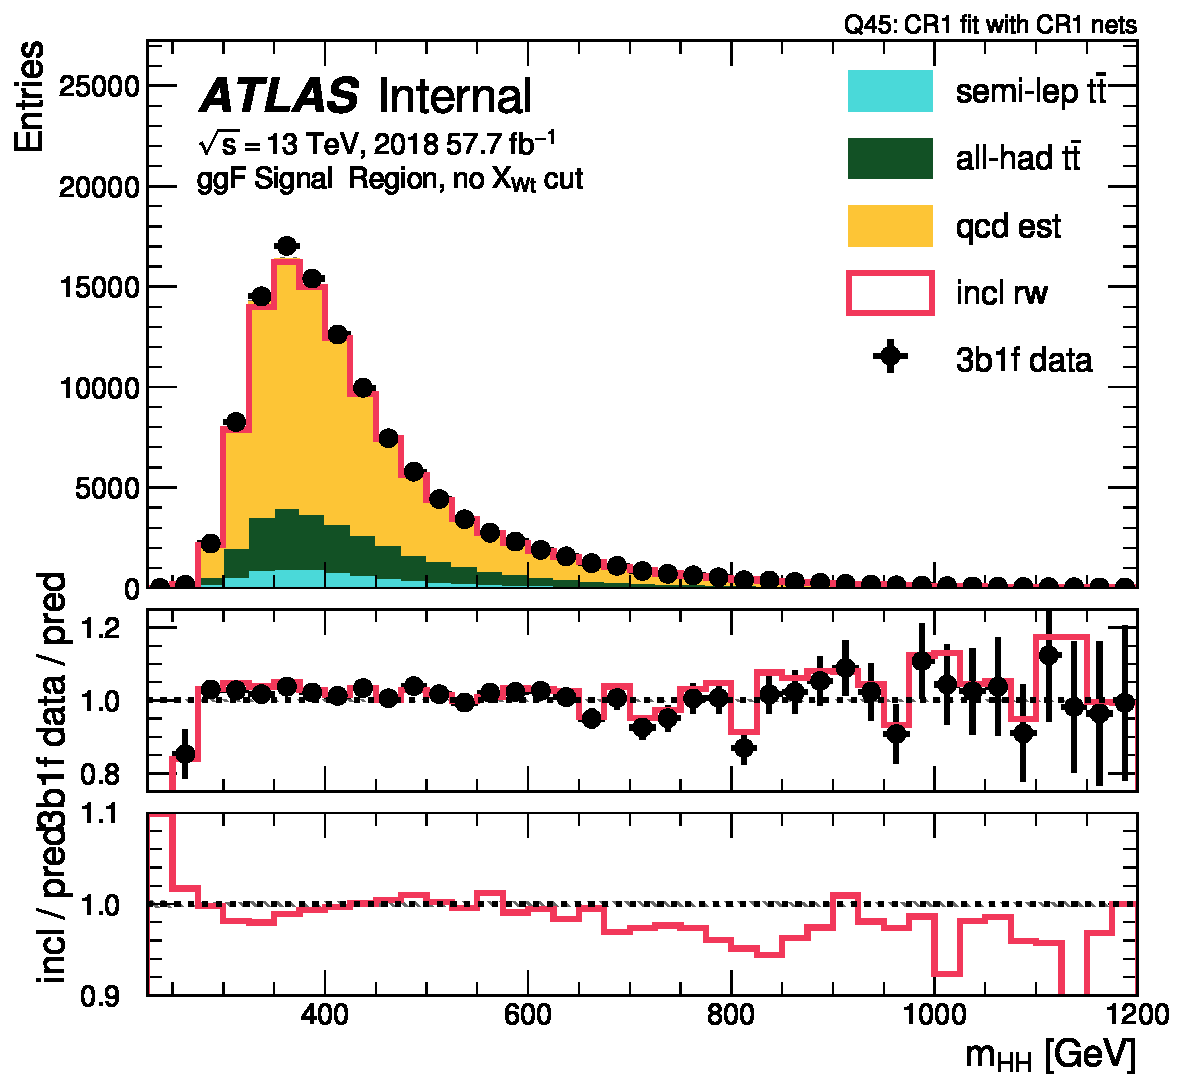
\includegraphics[width=.33\textwidth]{{figures/ttbar-rw/Q45/crFit_Xwtcut_1.5/m_hh_3b1f_SR_18}}}
\caption{3b1f SR evaluation using the CR1 fits}
\label{fig:mhh-sr-3b1f}
\end{figure}

\begin{figure}
\centering
\subfloat[2016]{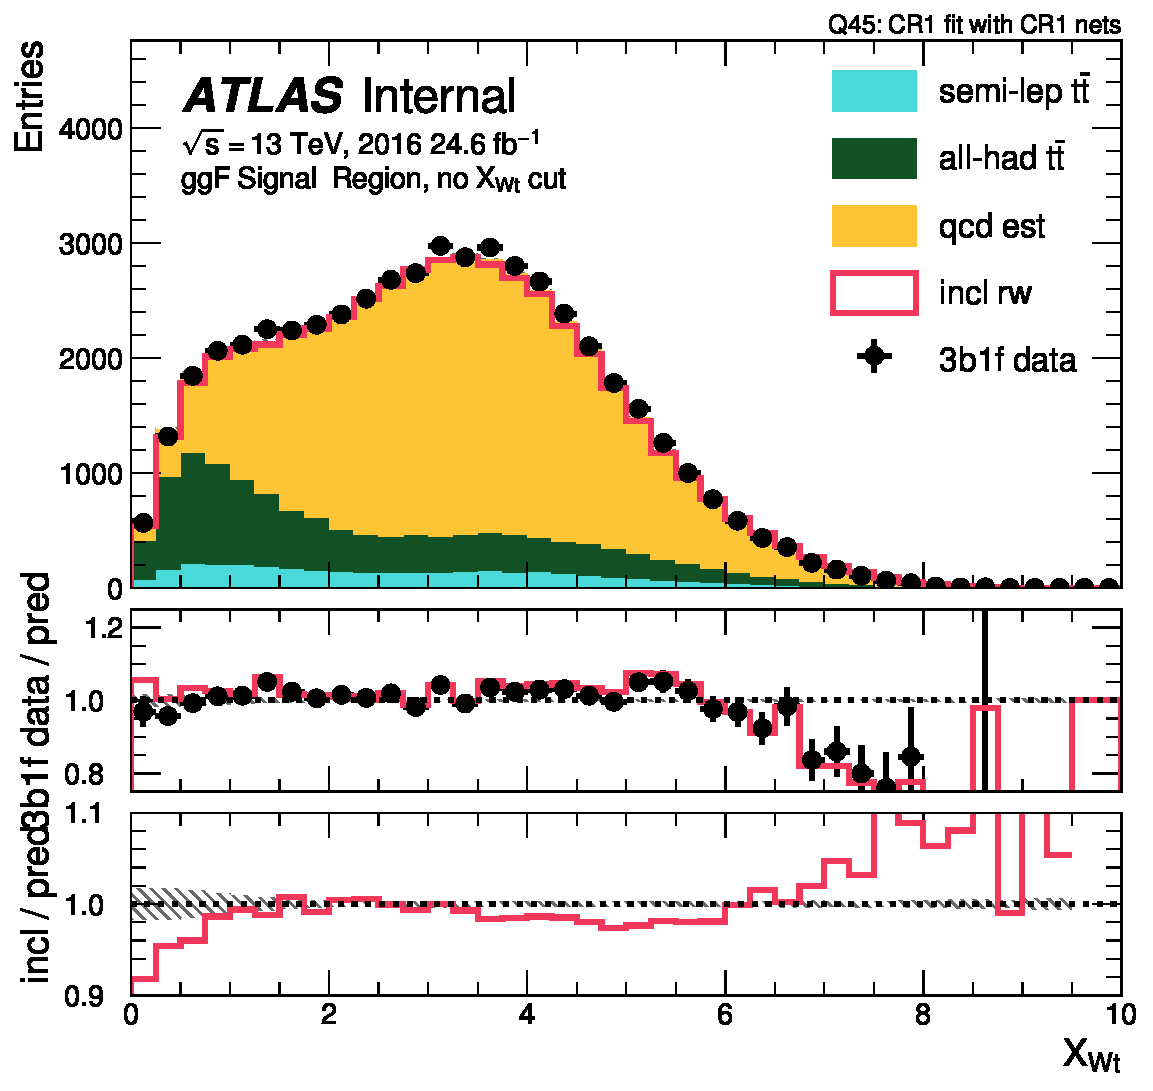
\includegraphics[width=.33\textwidth]{{figures/ttbar-rw/Q45/crFit_noXwtcut/X_wt_tag_3b1f_SR_16}}}
\subfloat[2017]{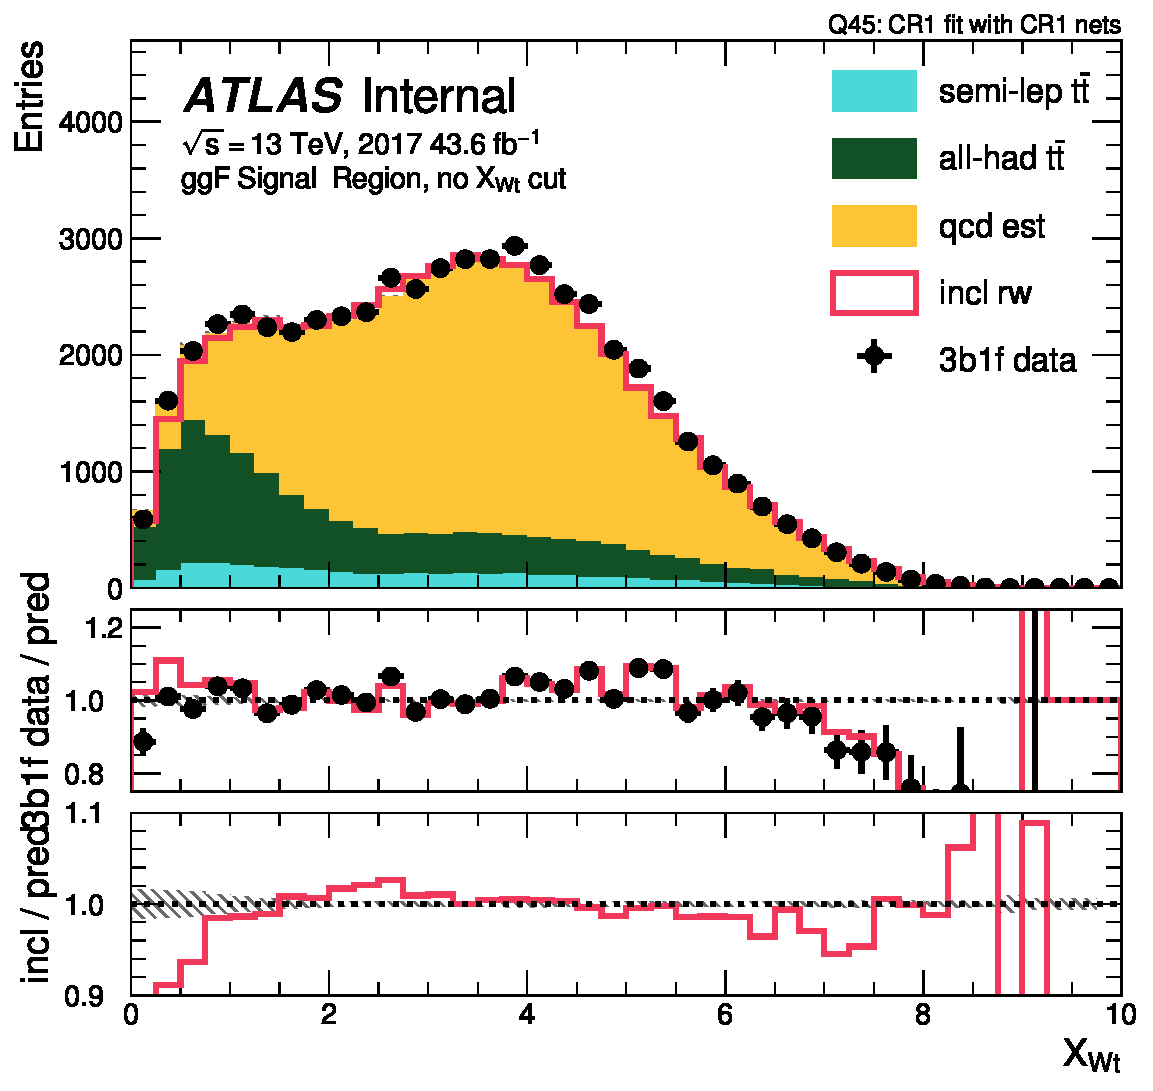
\includegraphics[width=.33\textwidth]{{figures/ttbar-rw/Q45/crFit_noXwtcut/X_wt_tag_3b1f_SR_17}}}
\subfloat[2018]{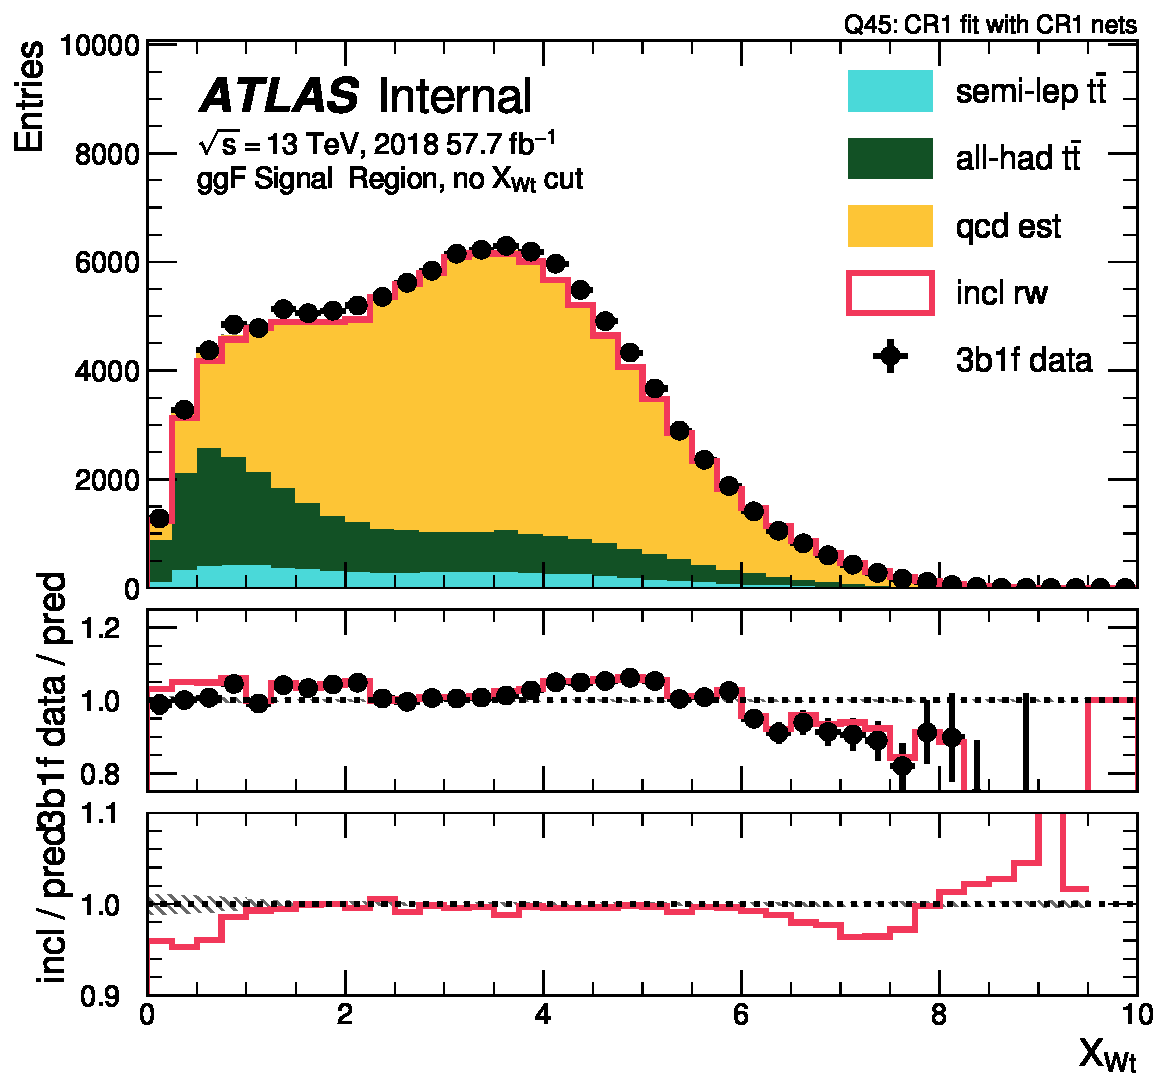
\includegraphics[width=.33\textwidth]{{figures/ttbar-rw/Q45/crFit_noXwtcut/X_wt_tag_3b1f_SR_18}}}
\caption{3b1f SR evaluation using the CR1 fits}
\label{fig:Xwt-sr-3b1f}
\end{figure}


\FloatBarrier
%\clearpage
\section{Pure QCD reweighting}
\label{pure-qcd}
We were a little bit confused why the template fits weren't working as well - and one hypothesis was that we were using the inclusively trained estimate to get the \ttbar template. In the next section, we show how to modify the loss function we used to get a pure QCD reweighting.

\subsection{Mathematical formulation}
\label{pure-qcd-math}

Rafael Teixeira de Lima developed this formalism, and this write-up closely follows his notes \cite{pure-qcd-Rafael}.

Let $R_{2b^{all} \rightarrow 4b^{all}}$  describe the inclusively trained reweighting. 
As demonstrated in \Fig{\ref{fig:ttbar-rw-graphic}}, this has two

\begin{equation}
R_{2b^{all} \rightarrow 4b^{all}} = \frac{\alpha_{4b}^{t\bar{t}} p_{4b}^{t\bar{t}} +  \alpha_{4b}^{Q} p_{4b}^{Q} }{ \alpha_{2b}^{t\bar{t}} p_{2b}^{t\bar{t}} +  \alpha_{2b}^{Q} p_{2b}^{Q}  }
\label{eq:rw-incl-defn}
\end{equation}
\noindent
where $p$ denotes the probability densities and $\alpha$ the corresponding normalizations. The subscripts 2\Pqb and 4\Pqb indicate the \Pqb-tagging requirement and the superscripts indicate 
the \ttbar and QCD (abbreviated ``Q'') physics samples.
Simplify the notation by letting $P_x^y = \alpha_x^y p_x^y$  so that \Eq{\ref{eq:rw-incl-defn}} becomes:

% I might want to take out the beginning bit and just start from the eqn below...

\begin{align*}
R_{2b^{all} \rightarrow 4b^{all}} &= \frac{P_{4b}^{t\bar{t}} +  P_{4b}^{Q} }{ P_{2b}^{t\bar{t}} +  P_{2b}^{Q}  } \\
&= \frac{P_{4b}^{t\bar{t}}}{ P_{2b}^{t\bar{t}} +  P_{2b}^{Q}  }  + \frac{P_{4b}^{Q} }{ P_{2b}^{t\bar{t}} +  P_{2b}^{Q}  }
\label{eq:rw-incl-short}
\end{align*}

We want to isolate the individual reweightings that we can derive:
\begin{align}
R_{2b^{all} \rightarrow 4b^{all}} &=  \frac{P_{4b}^{t\bar{t}}}{P_{2b}^{t\bar{t}} } \cdot \frac{1}{ 1 +  \frac{P_{2b}^{Q} }{P_{2b}^{t\bar{t}}} }  + \frac{P_{4b}^{Q} }{P_{2b}^{Q}} \cdot \frac{1}{ 1+ \frac{P_{2b}^{t\bar{t}}}{P_{2b}^{Q}}  }  \notag \\
&= \frac{P_{4b}^{t\bar{t}}}{P_{2b}^{t\bar{t}} } \cdot \frac{P_{2b}^{t\bar{t}}}{ P_{2b}^{t\bar{t}} +  P_{2b}^{Q} } + \frac{P_{4b}^{Q} }{P_{2b}^{Q}} \cdot \frac{P_{2b}^{Q} }{ P_{2b}^{Q} + P_{2b}^{t\bar{t}}  }  \notag \\
&= \textcolor{dodgerblue}{ \frac{P_{4b}^{t\bar{t}}}{P_{2b}^{t\bar{t}} }} \cdot \textcolor{mediumpurple}{ \frac{P_{2b}^{t\bar{t}}}{ P_{2b}^{t\bar{t}} +  P_{2b}^{Q} } } + \textcolor{hh:darkyellow}{ \frac{P_{4b}^{Q} }{P_{2b}^{Q}} } \cdot \left(1 - \textcolor{mediumpurple}{  \frac{P_{2b}^{t\bar{t}} }{ P_{2b}^{Q} + P_{2b}^{t\bar{t}}  } } \right)
\label{eq:rw-probs}
\end{align}

We can now identify:

\begin{itemize}
	\item \textcolor{dodgerblue}{$R_{2b^{t\bar{t}} \rightarrow 4b^{t\bar{t}}}$ } = $ \frac{P_{4b}^{t\bar{t}}}{P_{2b}^{t\bar{t}} }$: A MC based \ttbar reweighting 2\Pqb $\rightarrow$ 4\Pqb. 
	\item \textcolor{mediumpurple}{ $R_{2b^{t\bar{t}} \rightarrow 4b^{t\bar{t}}}$ } = $ \frac{P_{2b}^{t\bar{t}} }{ P_{2b}^{Q} + P_{2b}^{t\bar{t}}  }$ : Reweight the 2\Pqb data into the 2\Pqb \ttbar.
	\item \textcolor{hh:darkyellow}{ $ R_{2b^Q \rightarrow 4b^{Q}} $ }: a pure QCD reweighting -- what we want to solve for. 
\end{itemize}
\noindent
The first two reweightings in the list above are ones that we can easily derive.  $R_{2b^{all} \rightarrow 4b^{all}}$ is the current background estimate, so we can move forward to solve for \textcolor{hh:darkyellow}{ $ R_{2b^Q \rightarrow 4b^{Q}} $ }.
First, substitute these reweighting definitions into \Eq{\ref{eq:rw-probs}}: 

\begin{equation}
\textcolor{hh:darkpink}{ R_{2b^{all} \rightarrow 4b^{all}} } = 
\textcolor{dodgerblue}{R_{2b^{t\bar{t}} \rightarrow 4b^{t\bar{t}}} }  \cdot \textcolor{mediumpurple}{ R_{2b^{t\bar{t}} \rightarrow 4b^{t\bar{t}}} }  
+ \textcolor{hh:darkyellow}{ R_{2b^Q \rightarrow 4b^{Q}}  } \left(1 - \textcolor{mediumpurple}{ R_{2b^{t\bar{t}} \rightarrow 4b^{t\bar{t}} } }    \right). 
\end{equation}
\noindent
Rearrange to solve for $R_{2b^Q \rightarrow 4b^{Q}}$ :
\begin{equation}
\textcolor{hh:darkyellow}{ R_{2b^Q \rightarrow 4b^{Q}} } 
= 
\frac{
\textcolor{hh:darkpink}{ R_{2b^{all} \rightarrow 4b^{all}} }
- 
\textcolor{dodgerblue}{R_{2b^{t\bar{t}} \rightarrow 4b^{t\bar{t}}} }
\cdot 
\textcolor{mediumpurple}{ R_{2b^{t\bar{t}} \rightarrow 4b^{t\bar{t}}} } 
}
{1 - \textcolor{mediumpurple}{ R_{2b^{t\bar{t}} \rightarrow 4b^{t\bar{t}}} } }
\label{eq:qcd-rw}
\end{equation}

Now that we have a pure QCD reweighting, this gives a prescription for how to apply it to give a prediction for the 4b data:

\begin{equation}
P_{4b}^{all} = R_{2b^Q \rightarrow 4b^Q} \cdot \left( P_{2b}^{all} - P_{2b}^{t\bar{t}} \right) + P_{4b}^{t\bar{t}}.
\end{equation}

The first term $R_{2b^Q \rightarrow 4b^Q} \cdot \left( P_{2b}^{all} - P_{2b}^{t\bar{t}} \right)$ gives the piece for the QCD template, where we use the weights from \Eq{\ref{eq:qcd-rw}}. To get just the QCD template, we apply this reweighting formula to the 2\Pqb data and then subtract off the result of applying the reweighting to the 2\Pqb \ttbar MC.
The second term $P_{4b}^{t\bar{t}}$ gives the $t\bar{t}$ template, which we can just get using the $t\bar{t}$ MC.

\subsection{Experiments}
\label{pure-qcd-exp}

The following reweighting estimates just show a single training (instead of the whole machinery with 100 bootstraps) to get a sense for the scale of the problem and how much this method could help us. 
We'll want to fit the \Xwt template again, so the reweightings are derived in CR1 before the $\Xwt$ cut.

Using the neural network parameters from the inclusive reweighting (3 hidden layers with 50 neurons each) for the  
\textcolor{dodgerblue}{$R_{2b^{t\bar{t}} \rightarrow 4b^{t\bar{t}}}$ } and \textcolor{mediumpurple}{ $R_{2b^{t\bar{t}} \rightarrow 4b^{t\bar{t}}}$ } reweightings did not give good closure. The hyperparameters were re-optimized and a model with 3 hidden layers of 50, 25, and 10 neurons including batch normalization \cite{batch-norm} between the layers was found to work well. The closure on the reweighting variables (and \mhh) are shown in \Fig{\ref{mc-rw-d}} and \Fig{\ref{dat-to-mc-17}} for these two reweightings and demonstrates the confidence that we had that the individual reweightings going into \Eq{\ref{eq:qcd-rw}} were working nicely.

\begin{figure}
\centering
\includegraphics[width=\textwidth]{{figures/ttbar-rw/SWAN_plots/mc-rw-d-50-25-10/rwVars.pdf}}
\caption{\textcolor{dodgerblue}{$R_{2b^{t\bar{t}} \rightarrow 4b^{t\bar{t}}}$ } : The MC based 2\Pqb $\rightarrow$ 4\Pqb \ttbar reweighting. }
\label{fig:mc-rw-d}
\end{figure}

\begin{figure}
\centering
\includegraphics[width=\textwidth]{{figures/ttbar-rw/SWAN_plots/dat-to-mc-17-50-25-10/rwVars.pdf}}
\caption{\textcolor{mediumpurple}{ $R_{2b^{t\bar{t}} \rightarrow 4b^{t\bar{t}}}$ }: Reweighting 2\Pqb data $\rightarrow$ 2\Pqb \ttbar.}
\label{fig:dat-to-mc-17}
\end{figure}

Although it seemed like the new reweighting were optimized well, when I applied the weights from \Eq{\ref{eq:qcd-rw}}, the resulting \Xwt distribution had a very discontinuous QCD template in the \Xwt $<$ 1.5 region, motivating us to dive in and understand what the issues were:

\begin{itemize}
	\item When \textcolor{mediumpurple}{ $R_{2b^{t\bar{t}} \rightarrow 4b^{t\bar{t}}}$ } is very slightly larger than 1, we get large negative amplification in the weight from the denominator going to zero.
	\item Sometimes we also got unphysically large weights for the \textcolor{dodgerblue}{$R_{2b^{t\bar{t}} \rightarrow 4b^{t\bar{t}}}$ } reweighting, suggesting that this was a region of low support for the data the 2b distribution)
	\item Sometimes the subtraction in the numerator caused the weight to become negative and was accompanied by a large amplification from the denominator being small as well.
\end{itemize}

%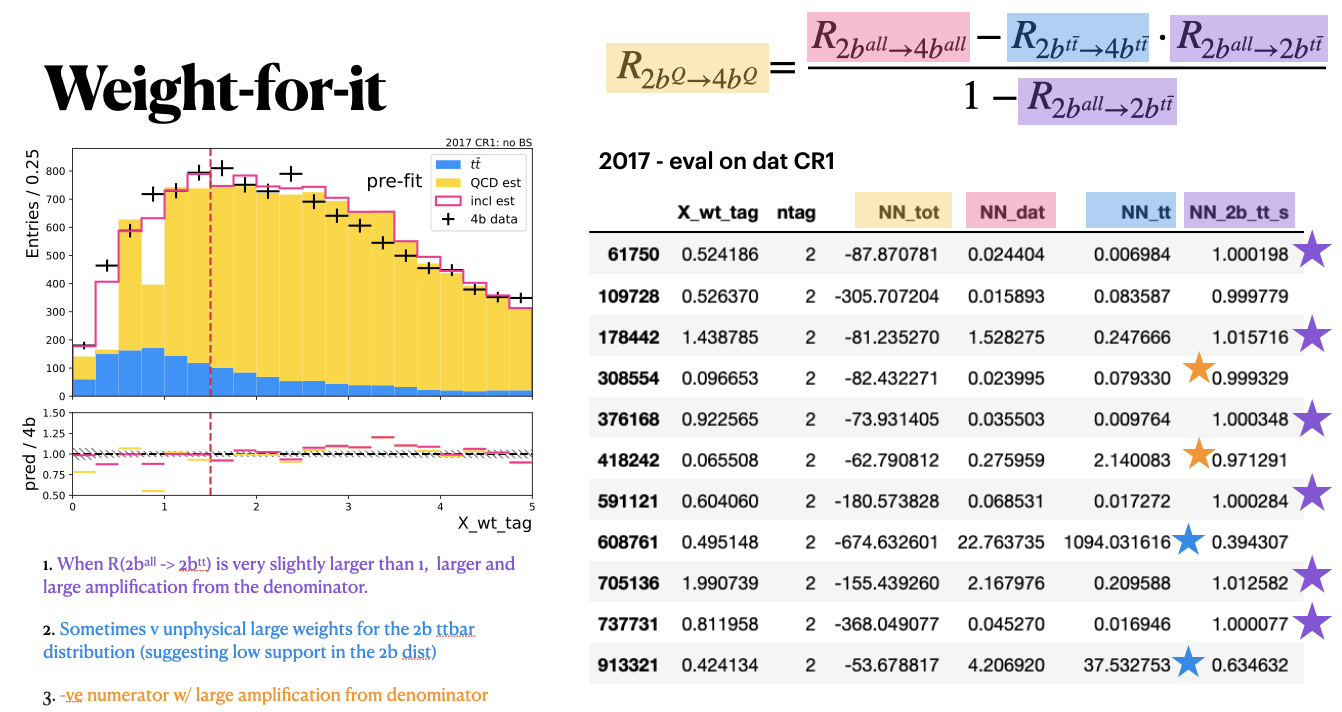
\includegraphics[width=\textwidth]{{figures/my_dihiggs/ttbar-weight-for-it}}

To fix the odd shaped qcd template issue, we removed the unphysical weights by cutting out the events with a weight more than 10 $\sigma$ away from the mean. The resulting pre-fit templates for all of the years are shown in the right-hand column of \Fig{\ref{fig:pure-qcd-fits}}, a by-eye reasonable template for modeling the pure QCD distribution.  

We then the 2 components to the \Xwt shape inside in CR1 and check the agreement.
\Tab{\ref{tab:pure-qcd-fits}} shows the normalizations for the pure QCD fits, and the left-hand column of \Fig{\ref{fig:pure-qcd-fits}} shows the post-fit plots.

\begin{table}[h]
	\centering
	\setlength\extrarowheight{5pt}
	\begin{tabular}{c|c|c|c}
	{} & {16} & {17} & {18}  \\
	\hline
	\textcolor{dodgerblue}{\textbf{$\alpha_{t\bar{t}}$}} & $1.27 \pm 0.11$     & $1.84 \pm 0.09$     &  $0.66 \pm 0.08$ \\
	\textcolor{hh:darkyellow}{\textbf{$\alpha_{QCD}$}}& $0.950 \pm 0.018$ & $0.913 \pm 0.014$ &  $1.012 \pm 0.013$ \\
	\end{tabular}
	\caption{Fitted normalizations for the \ttbar and QCD templates with the pure QCD reweighting.}
	\label{tab:pure-qcd-fits}
\end{table}

\begin{figure}
\centering
\subfloat[2016 pre-fit]{
	\includegraphics[width=.48\textwidth]{{figures/ttbar-rw/SWAN_plots/ttbar-2comp-16-models-50-25-10/ttbar_2_comp_prefit.pdf}}
}
\subfloat[2016 post-fit]{
	\includegraphics[width=.48\textwidth]{{figures/ttbar-rw/SWAN_plots/ttbar-2comp-16-models-50-25-10/ttbar_2_comp_postfit.pdf}}
} \\
\subfloat[2017 pre-fit]{
	\includegraphics[width=.48\textwidth]{{figures/ttbar-rw/SWAN_plots/ttbar-2comp-17-models-50-25-10/ttbar_2_comp_prefit.pdf}}
}
\subfloat[2017 post-fit]{
	\includegraphics[width=.48\textwidth]{{figures/ttbar-rw/SWAN_plots/ttbar-2comp-17-models-50-25-10/ttbar_2_comp_postfit.pdf}}
} \\
\subfloat[2018 pre-fit]{
	\includegraphics[width=.48\textwidth]{{figures/ttbar-rw/SWAN_plots/ttbar-2comp-18-models-50-25-10/ttbar_2_comp_prefit.pdf}}
}
\subfloat[2018 post-fit]{
	\includegraphics[width=.48\textwidth]{{figures/ttbar-rw/SWAN_plots/ttbar-2comp-18-models-50-25-10/ttbar_2_comp_postfit.pdf}}
}
\caption{\Xwt distributions in CR1 with the pre-fit (left) and post-fit (right) plots, compared to the 4b CR1 data.}
\label{fig:pure-qcd-fits}
\end{figure}

%Although a follow-up step would be to do similar fits studies as conducted in \Sect{\ref{sec:ttbar-fits}}, for the timescale of the Run~2 analysis, a pure QCD estimate was not feasible. 
I'm presenting the results here because I think it is an interesting study, and in the context of the approval processes for the analyses, how to account for $t\bar{t}$ or single Higgs backgrounds in the reweighting came up a lot. 
However, in terms of where is most useful to invest time in the next iteration, in \Sect{tbd} I will show that accounting for \ttbar separately is also possible in other direct density estimation methods, and I personally think these are more promising for pursuing in the future, partially because although the pure QCD reweighting is mathematically elegant, implementing it in practice wasn't quite as trivial since getting a final weight that was reasonable when accounting for the weights of all of these separate pieces was rather non-trivial.
%Furthermore, although this procedure shows how to reweight with separate components, we still need to derive / calculate a shape systematic for the differences between the CR where the weights are derived and the SR where they will ulitmately be applied.

\subsection{Outlook}
\label{pure-qcd-outlook}
After Run~3, our dataset size will \emph{double}, making the intricacies of how we treat the separate components of our background estimate even more relevant.
Although we showed several ideas for how to use the power of simulation, it wasn't deemed necessary for this current iteration of the physics analysis in terms of the background modelling, but, as we transition away from setting limits and into the realm of signal extraction, the import of well constraining each component of the background only grows.
This chapter focused on $t\bar{t}$ background, and even though it is only 10\% of our background, it is 100x as large as our HH signal. Another background we will start to care about more in the future is single Higgs background. Our single Higgs yield in the 4b SR is 3x the SM HH signal. 
The $bb\gamma \gamma$ analysis already includes the single Higgs background in their background modelling for the limit extraction, but the same methods from \Sect{\ref{pure-qcd-math}} can be used to use MC to separately model the single Higgs background and is good in the future to HHarmonize with the other channels in our quest to extract the HH signal.



